\documentclass{IFES-beamer}
\usepackage{url}
\usepackage{hyperref}

% --------------------------------------------------- %
%                  Presentation info	              %
% --------------------------------------------------- %
\title[Presentation Template]{Modelling Ecological Populations}
\subtitle{Game Theory Project}
\author{Ganga $\&$ Deddy \\ EE15B025 $\&$ EE15B125}
\institute[IFES]{
  Dynamic Games : Theory and Applications\\
  IIT Madras
}
\date{\today}
\logo{

\includegraphics[scale=0.75]{logo.jpeg}
}
\subject{Presentation subject} % metadata

% --------------------------------------------------- %
%                    Title + Schedule                 %
% --------------------------------------------------- %

\begin{document}

\begin{frame}
  \titlepage
\end{frame}

\begin{frame}{Schedule}
  \tableofcontents
\end{frame}

% --------------------------------------------------- %
%                      Presentation                   %
% --------------------------------------------------- %

%%%%%%%%%%%%%%%%%%%%%%%%%%%%%%%%%%%%%%%%%%%%%%%%%%%%%%%%%%%%%%%%%%%%%%
\section{Overview}

        
    %----------------------------------------------------------
    \begin{frame}{Reinforcement Learning}
        \begin{itemize}
            \item Provides a formalism for behavior
            \item Obtained from behavioral psychology
            \item Helpful for modelling ecological populations
        \end{itemize}
        \begin{figure}[H]
                \centering
                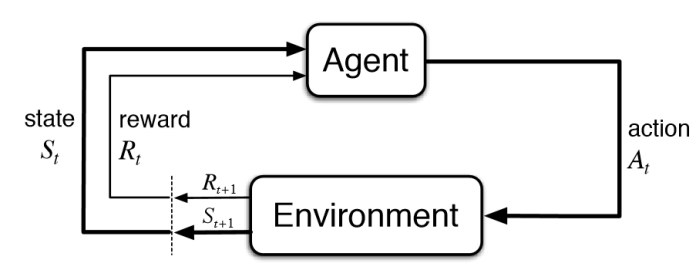
\includegraphics[scale=0.4]{Images/RL-intro.png}
                \caption{Reinforcement Learning}
                \label{fig:RL}
            \end{figure}
    \end{frame}
            
    %----------------------------------------------------------
    \begin{frame}{Methods in Reinforcement Learning}
        \begin{itemize}
            \item Policy Gradient
                \begin{itemize}
                    \item Players have policies (actions)
                    \item Optimize in the policy space
                    \item Gradient Ascent 
                    \item Episodic reward
                    \item $\pi(a_i, \theta)$ = Policy parameterized by $\theta$. \\
                    $\theta$ represents the parameters of our neural network.
                    \item $$\Delta \theta = \alpha_t r_r \frac{d}{d \theta} \pi(a_t, \theta_t)$$
                \end{itemize}
            \item Multi-Armed Bandits
                \begin{itemize}
                    \item Players pick from k arms
                    \item Find the best arm to pull
                \end{itemize}
        \end{itemize}
    \end{frame}

    % \begin{frame}{Reinforcement Learning for Game Theory - Good or Bad?}
    %     \begin{itemize}
    %         \item Good
    %             \begin{itemize}
    %                 \item Simulates dumb players well (those who didn't take a course in game theory)
    %                 \item Solution guaranteed to stay at evolutionary stable states
    %             \end{itemize}
    %         \item Bad
    %             \begin{itemize}
    %                 \item Mathematical guarantees don't hold
    %                 \item Dynamic environment
    %             \end{itemize}
    %     \end{itemize}
    % \end{frame}
    

    %$$$$$$$$$$$$$$$$$$$$$$$$$$$$$$$$$$$$$$$$$$$$$$$$$$$$$$$$$$$$$$
    \subsection{Hawk-Dove Game}
        %----------------------------------------------------------
        \begin{frame}{Hawk-Dove Game}
            \begin{itemize}
                \item What is it?
                    \begin{itemize}
                        \item Models interaction within same species
                        \item Sharing of resources
                    \end{itemize}
                \item Pay-off matrix : \\
                    \begin{table}[H]
                      \begin{center}
                        \begin{tabular}{|c|c|c|} % <-- Alignments: 1st column left, 2nd middle and 3rd right, with vertical lines in between
                        \hline
                        & Hawk & Dove\\
                          \hline
                          Hawk & $\frac{B-C}{2}, \frac{B-C}{2}$ & $B, 0$ \\
                          \hline
                          Dove & $0, B$ & $\frac{B}{2}, \frac{B}{2}$ \\
                          \hline
                        \end{tabular}
                      \end{center}
                    \end{table}
                \item B < C ; (B=6, C=10 in our expts)
                    \begin{table}[H]
                      \begin{center}
                        \begin{tabular}{|c|c|c|} % <-- Alignments: 1st column left, 2nd middle and 3rd right, with vertical lines in between
                        \hline
                        & Hawk & Dove\\
                          \hline
                          Hawk & -2, -2 & 6, 0 \\
                          \hline
                          Dove & 0, 6 & 3, 3 \\
                          \hline
                        \end{tabular}
                      \end{center}
                    \end{table}
                \item The pay-off of player i is denoted by $u_i(s_i, s_j)$
            \end{itemize}
        \end{frame}
    
        %----------------------------------------------------------
        \begin{frame}{Nash Equilibria : Hawk-Dove Game}
        \begin{itemize}
                \item 3 nash equilibria
                \item 2 pure + 1 mixed
        \end{itemize}
            \begin{figure}
                \centering
                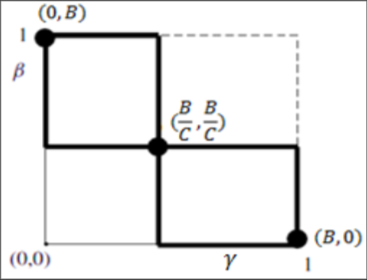
\includegraphics[scale=0.3]{Images/nash_eqm.png}
                \caption{Nash Equilibria in a Hawk-Dove Game\cite{Essam}}
                \label{fig:my_label}
            \end{figure}
        \end{frame}
        
        
        %----------------------------------------------------------
        \begin{frame}{Modified Hawk-Dove Game}
            \begin{itemize}
                \item A population of N players
                \item Each player can be a hawk or a dove
                \item Pay-off decided based on interaction with population
                \item Pay-off of player i in the population is denoted by $u_i(s_i, s_{-i})$
            \end{itemize}
            \begin{figure}[H]
                \centering
                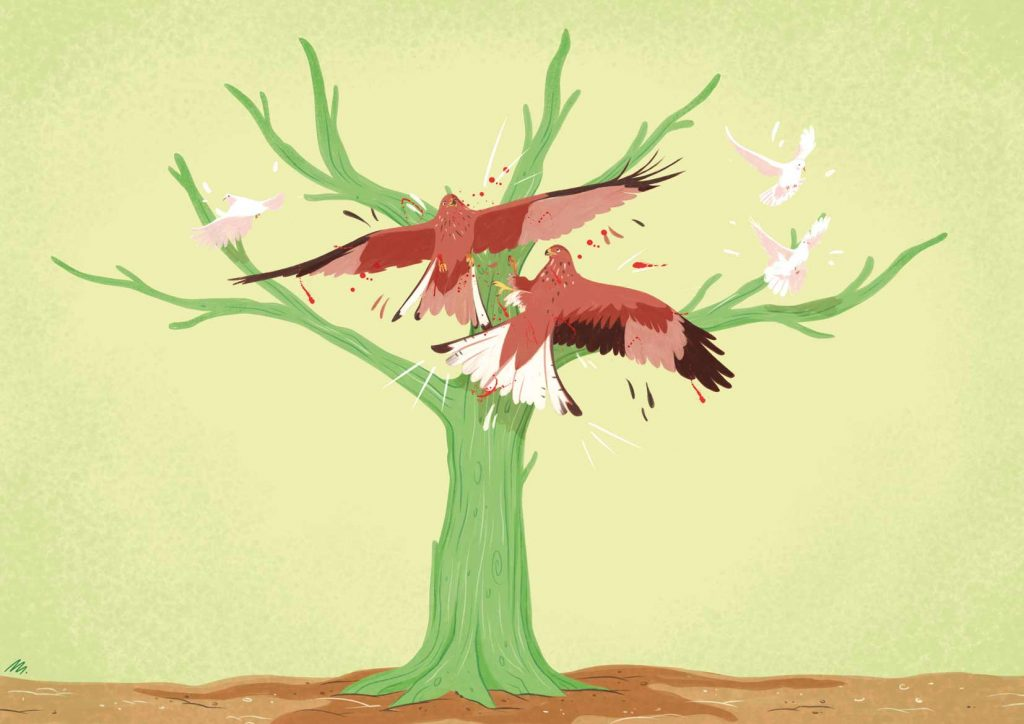
\includegraphics[scale=0.15]{Images/hawk_dove.jpg}
                \caption{N-player hawk-dove game}
            \end{figure}
        \end{frame}
        
        %----------------------------------------------------------
        \begin{frame}{From RL Perspective}
            \begin{figure}[H]
                \centering
                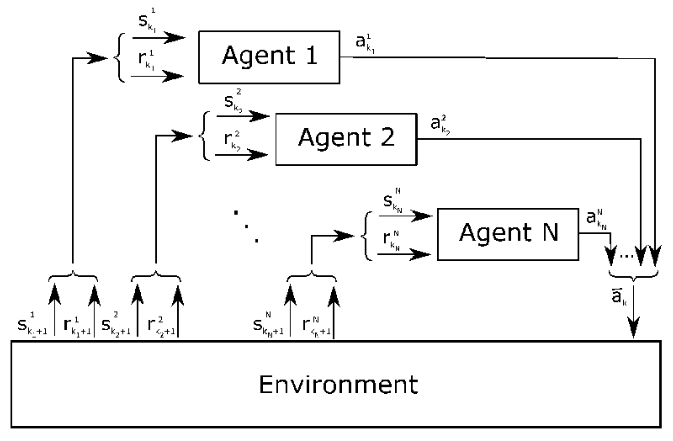
\includegraphics[scale=0.3]{Images/Multi_RL.png}
                \caption{N-player hawk-dove game (Ref : \href{https://towardsdatascience.com/modern-game-theory-and-multi-agent-reinforcement-learning-systems-e8c936d6de42}{MARL})}
            \end{figure}
        \end{frame}
        
        %----------------------------------------------------------
        \begin{frame}{Measuring individual pay-off}
            \begin{enumerate}
                \item Playing against the field $$u_i(s_i, s_{-i}) = \frac{1}{N} \sum_{\forall j \neq i} u_i(s_i, s_j)$$
                \item Playing against a group $M_j$ $$u_i(s_i, s_{-i}) = \frac{1}{|M_j|} \sum_{j \in M_j} u_i(s_i, s_j)$$
                \item Pair-wise contest \\(Player j chosen randomly by nature) $$u_i(s_i, s_{-i}) = u_i(s_i, s_j)$$
            \end{enumerate}
        \end{frame}
        
        %----------------------------------------------------------
        \begin{frame}{A better understanding of its significance during convergence}
            \begin{figure}[H]
                \centering
                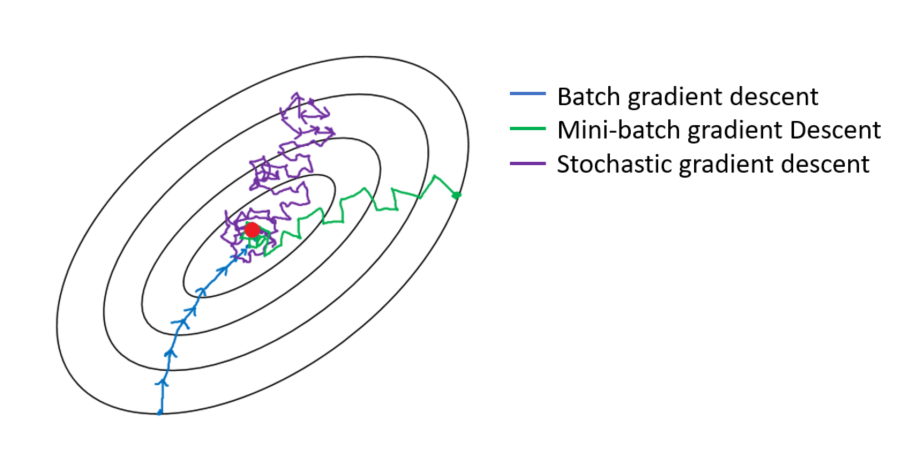
\includegraphics[scale=0.25]{Images/GD.png}
                \caption{Convergence comparison of the three methods of calculating individual pay-offs : Playing against the field, Playing against a group and Pair-wise contest respectively}
                \label{fig:GD}
            \end{figure}
        \end{frame}
        
        %----------------------------------------------------------
        \begin{frame}{Some Definitions}
            \begin{itemize}
                \item \textbf{Static Games}: A static game is one in which all players make decisions (or select a strategy) simultaneously, without knowledge of the strategies that are being chosen by other players. Even though the decisions may be made at different points in time, the game is simultaneous because each player has no information about the decisions of others; thus, it is as if the decisions are made simultaneously.
                \item \textbf{Stage Games}: A Stage Game is a game that arises in certain stage of a static game. In other words, the rules of the games depend on the specific stage. The prisoner’s dilemma is a classic example of stage game
            \end{itemize}
        \end{frame}
        

%%%%%%%%%%%%%%%%%%%%%%%%%%%%%%%%%%%%%%%%%%%%%%%%%%%%%%%%%%%%%%%%%%%%%%
\section{Models}
    %$$$$$$$$$$$$$$$$$$$$$$$$$$$$$$$$$$$$$$$$$$$$$$$$$$$$$$$$$$$$$$
    \subsection{Non-Cooperative games}
        %----------------------------------------------------------
        \begin{frame}{NN Model Multi-brain}
                \begin{itemize}
                    \item Selfish agents
                    \item Policy Gradient update
                    \item Players have stochastic strategies, but play pure strategies
                \end{itemize}
                \begin{figure}[H]
                \centering
                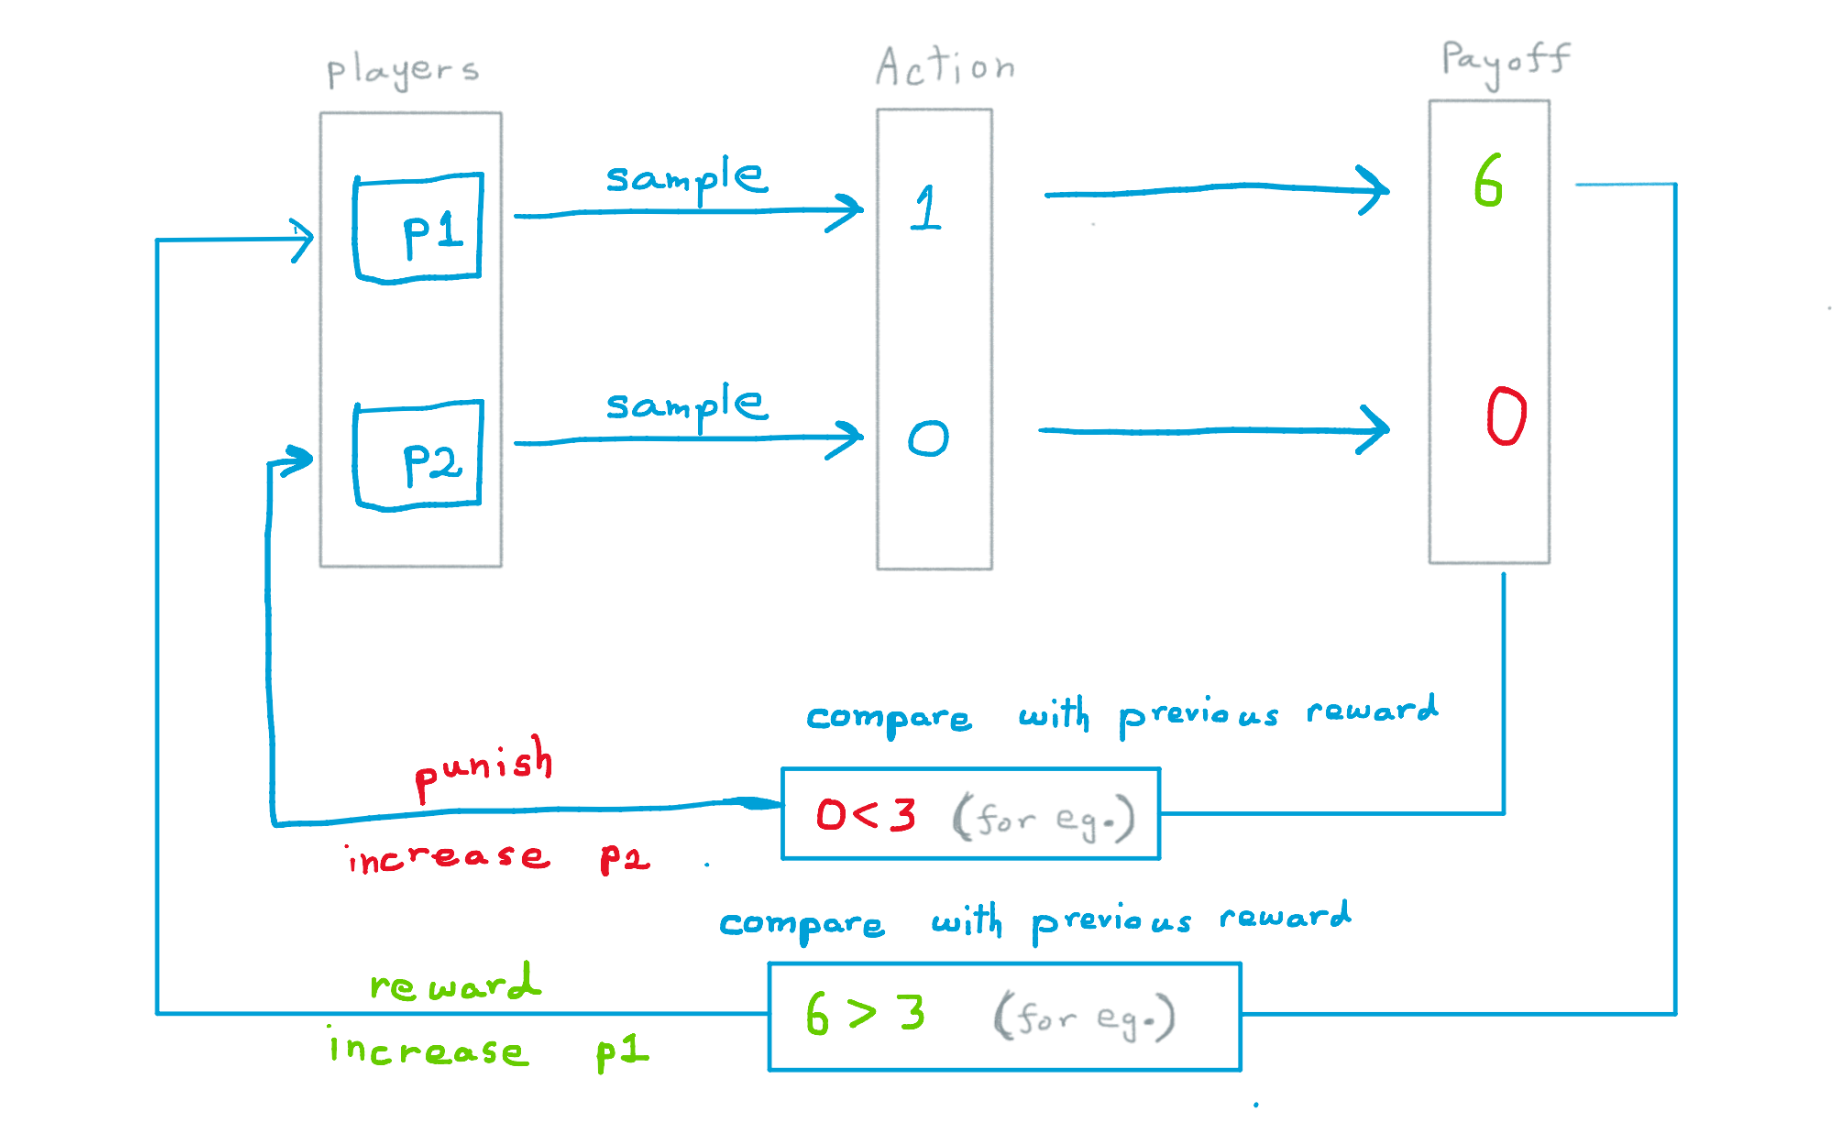
\includegraphics[scale=0.35]{Images/no_coop.png}
                \caption{RL mechanism for pairwise contests}
            \end{figure}
        \end{frame}

        %----------------------------------------------------------
        \begin{frame}{Pairwise contests}
        \begin{enumerate}
            \item Players are matched randomly
            \item Strategies drawn from Bernoulli distribution
        \end{enumerate}
            \begin{figure}[H]
                \centering
                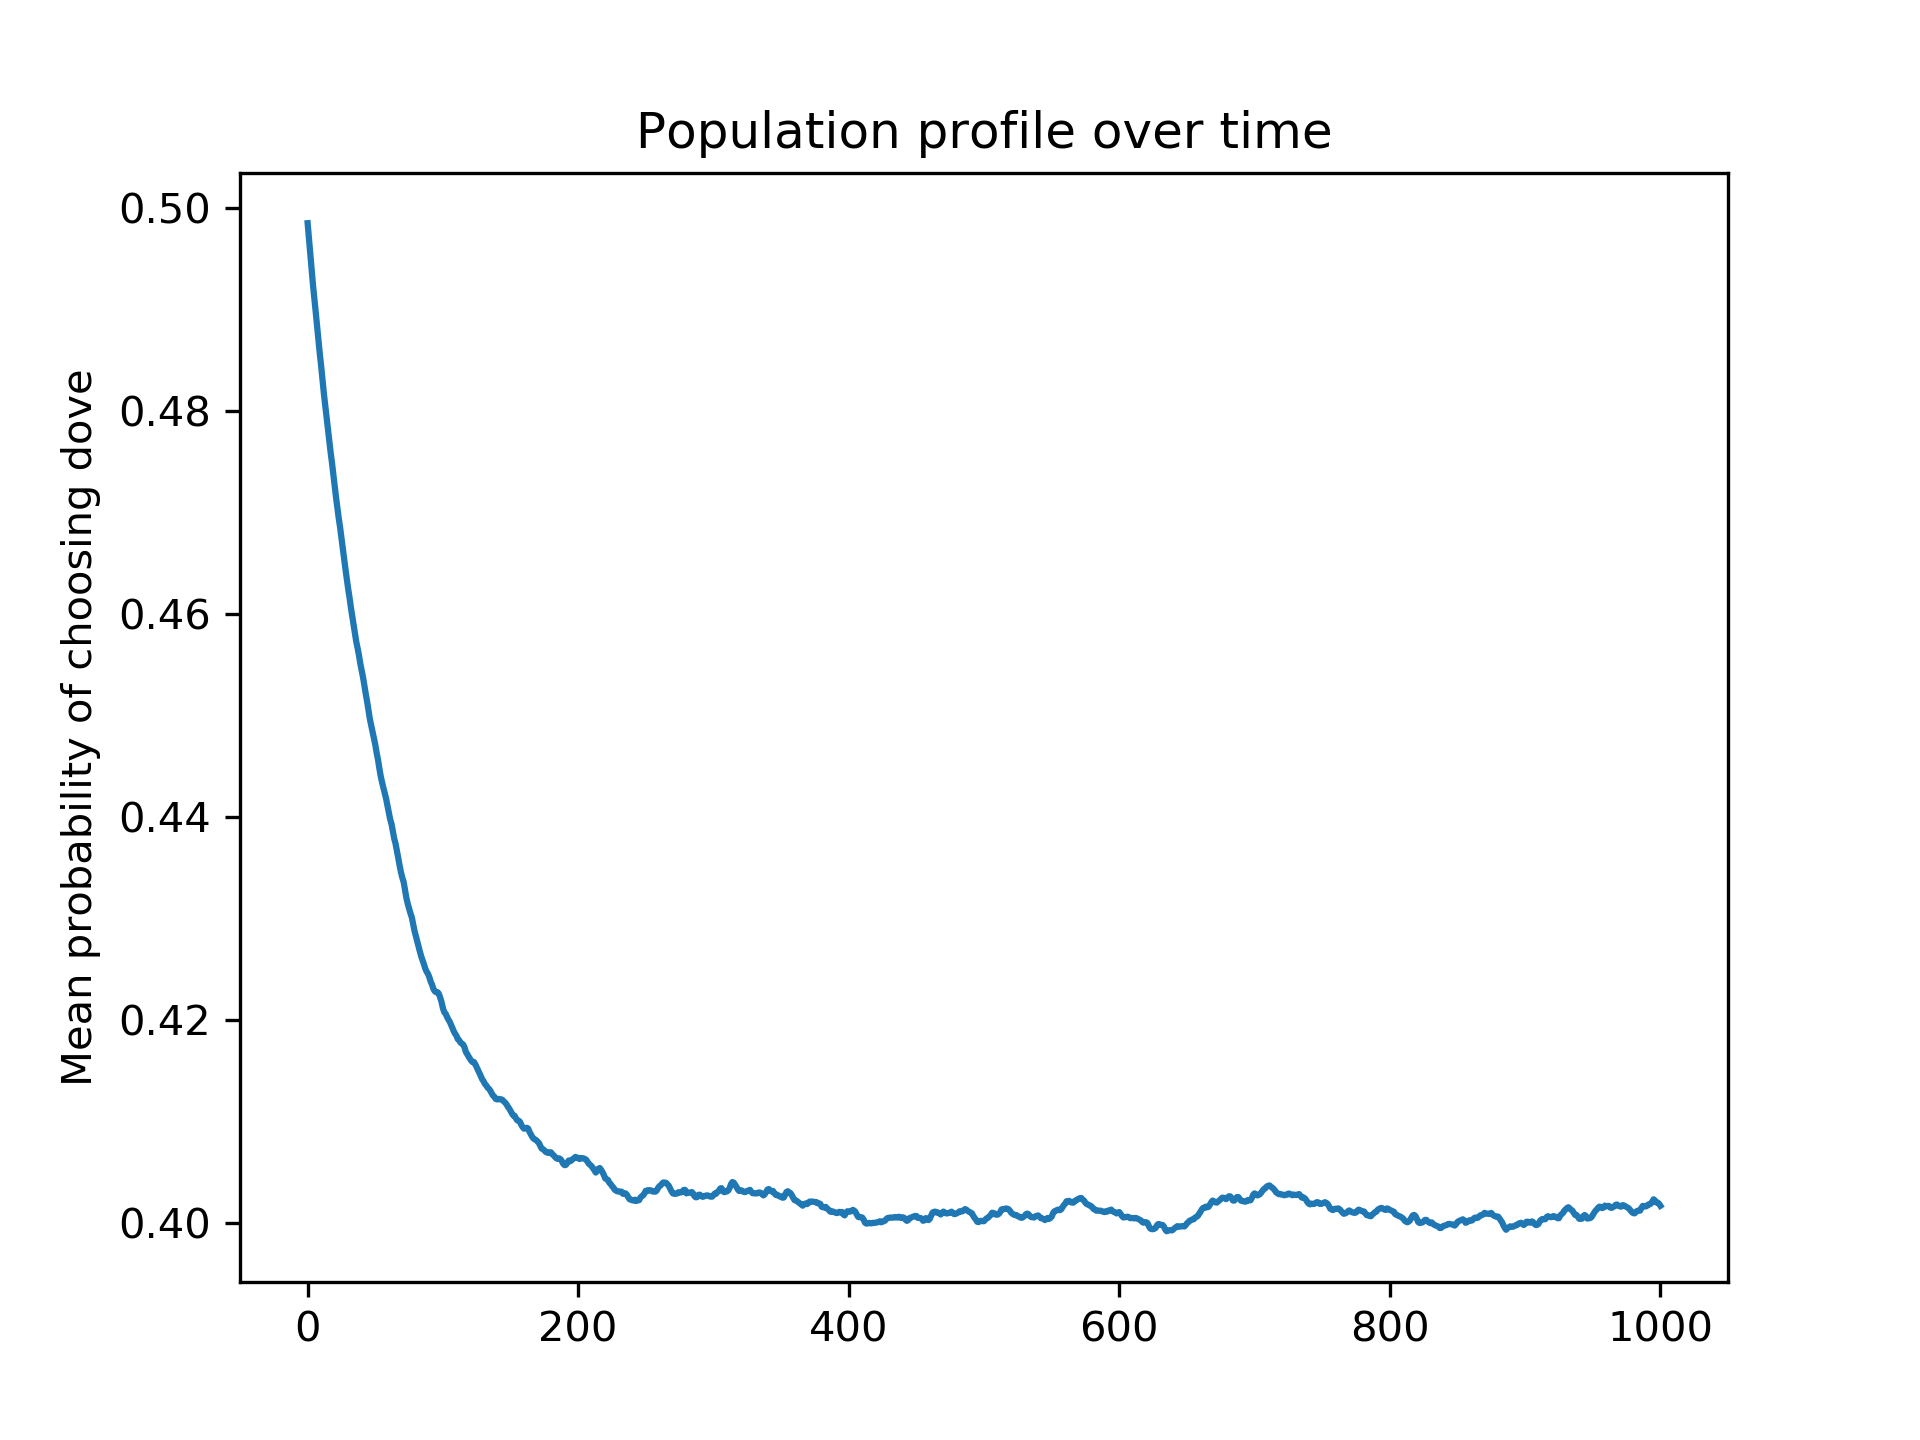
\includegraphics[scale=0.4]{Images/multi_brain_pair.png}
                \caption{State of population over time: pairwise contests}
                \label{fig:GD}
            \end{figure}
        \end{frame}
        
                
        %----------------------------------------------------------
        \begin{frame}{Playing against Field}
            \begin{enumerate}
                \item Strategies drawn from Bernoulli distribution
                \item Payoff obtained against population profile
                \item Population converges faster (sort of)
            \end{enumerate}
                \begin{figure}[H]
                \centering
                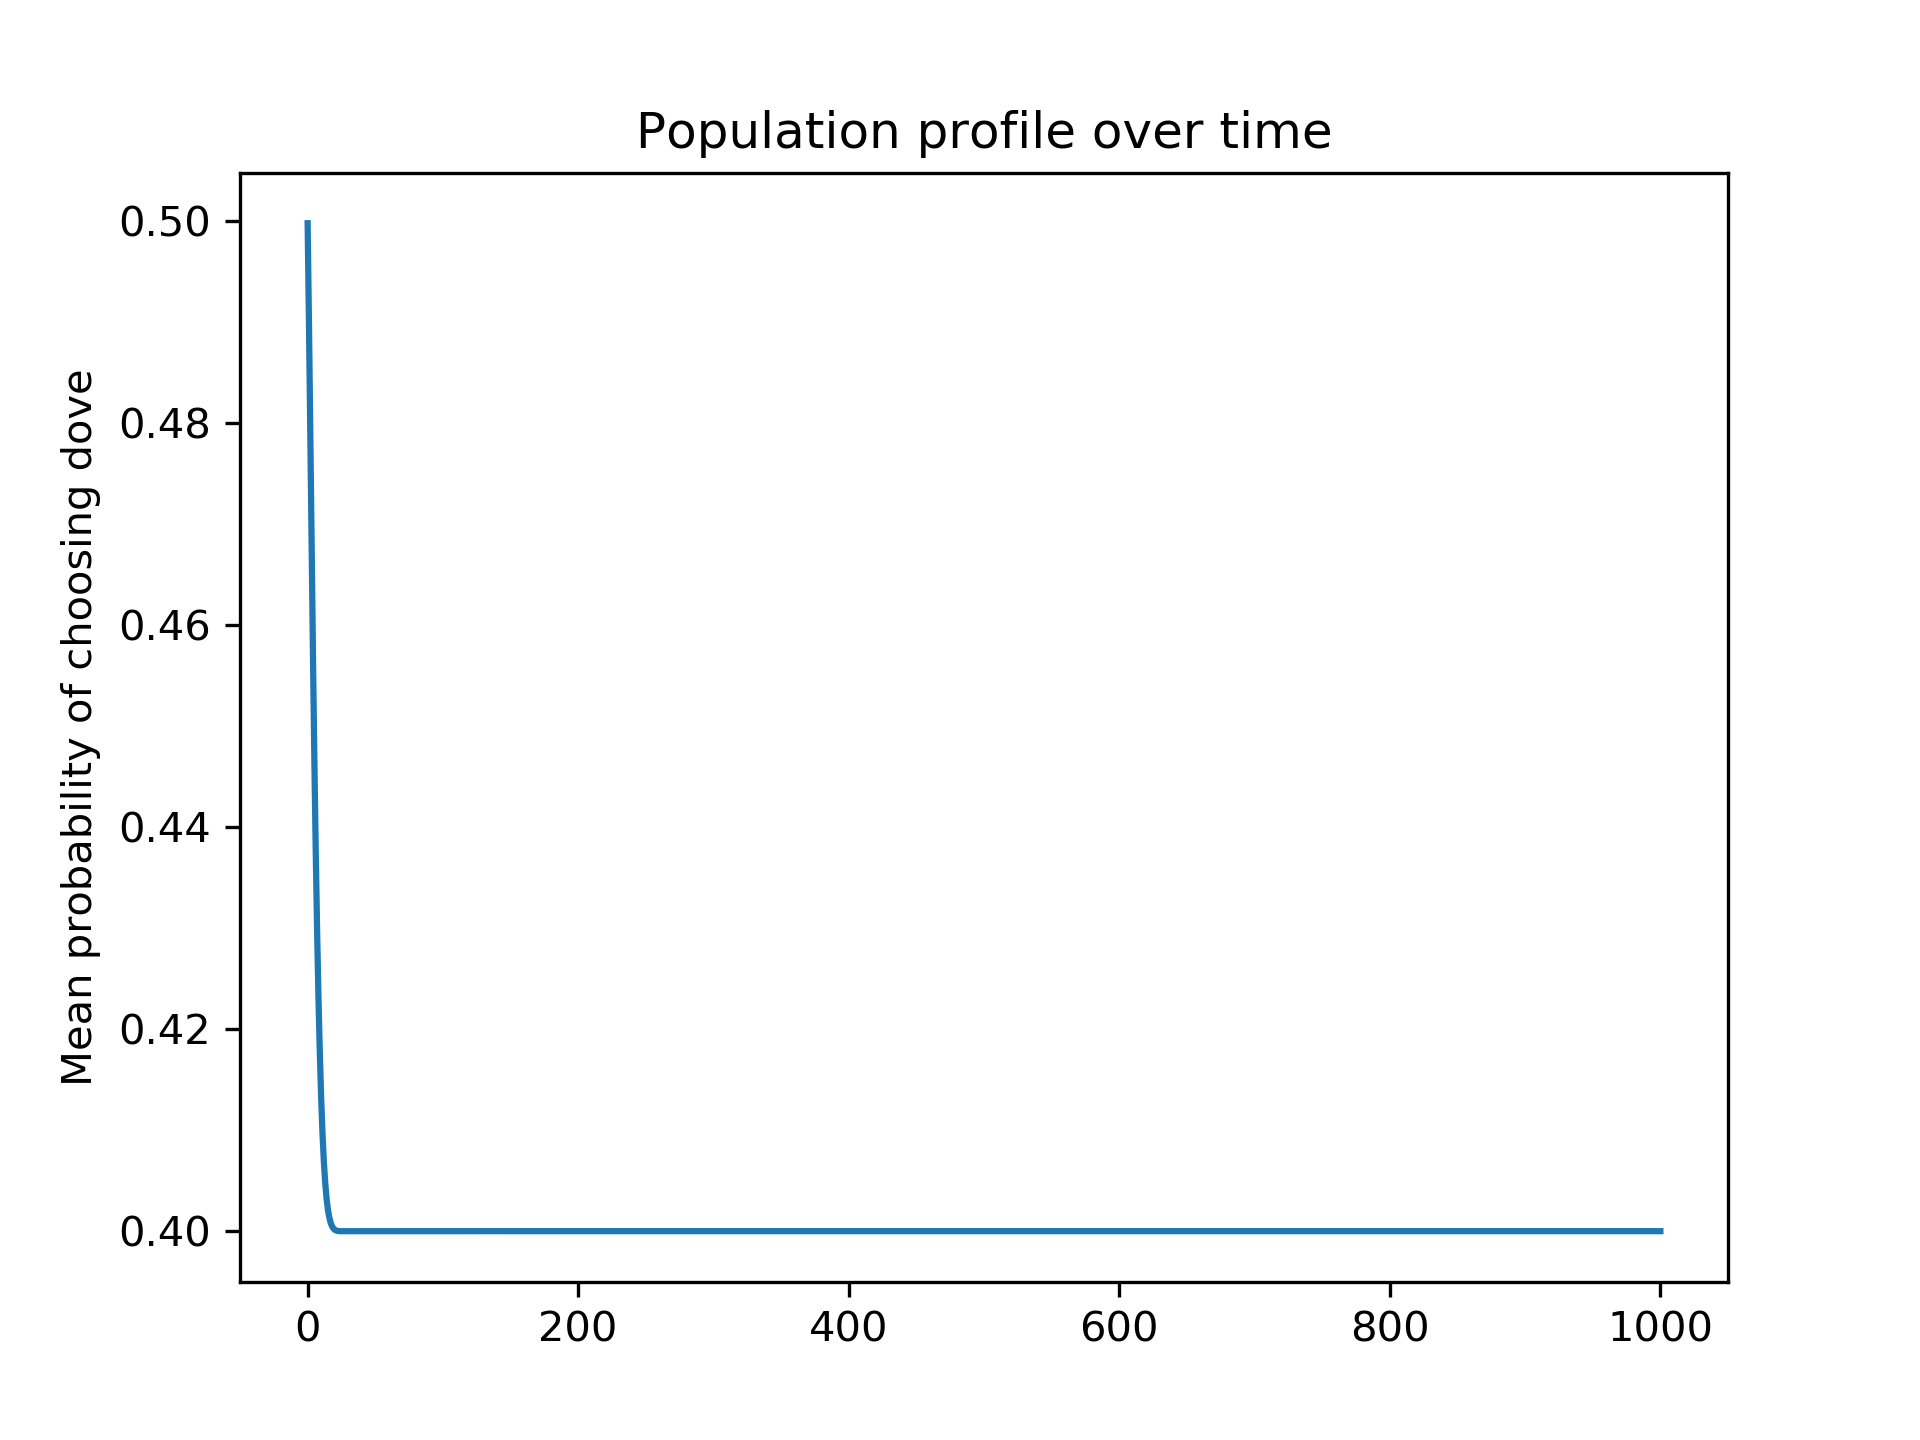
\includegraphics[scale=0.4]{Images/pop_profile_field.png}
                \caption{State of population over time: against the field}
                \label{fig:GD}
            \end{figure}
        \end{frame}
        
    
    
    %$$$$$$$$$$$$$$$$$$$$$$$$$$$$$$$$$$$$$$$$$$$$$$$$$$$$$$$$$$$$$$
    \subsection{NN Model - Code of Conduct}
        %----------------------------------------------------------
        \begin{frame}{NN Model - Code of Conduct}
            \begin{itemize}
                \item Players still selfish...
                \item But agree to a "code of conduct" or Rules of Engagement (RoE)
                \item Code of conduct updated by each player in turns
            \end{itemize}
            \begin{figure}[H]
                \centering
                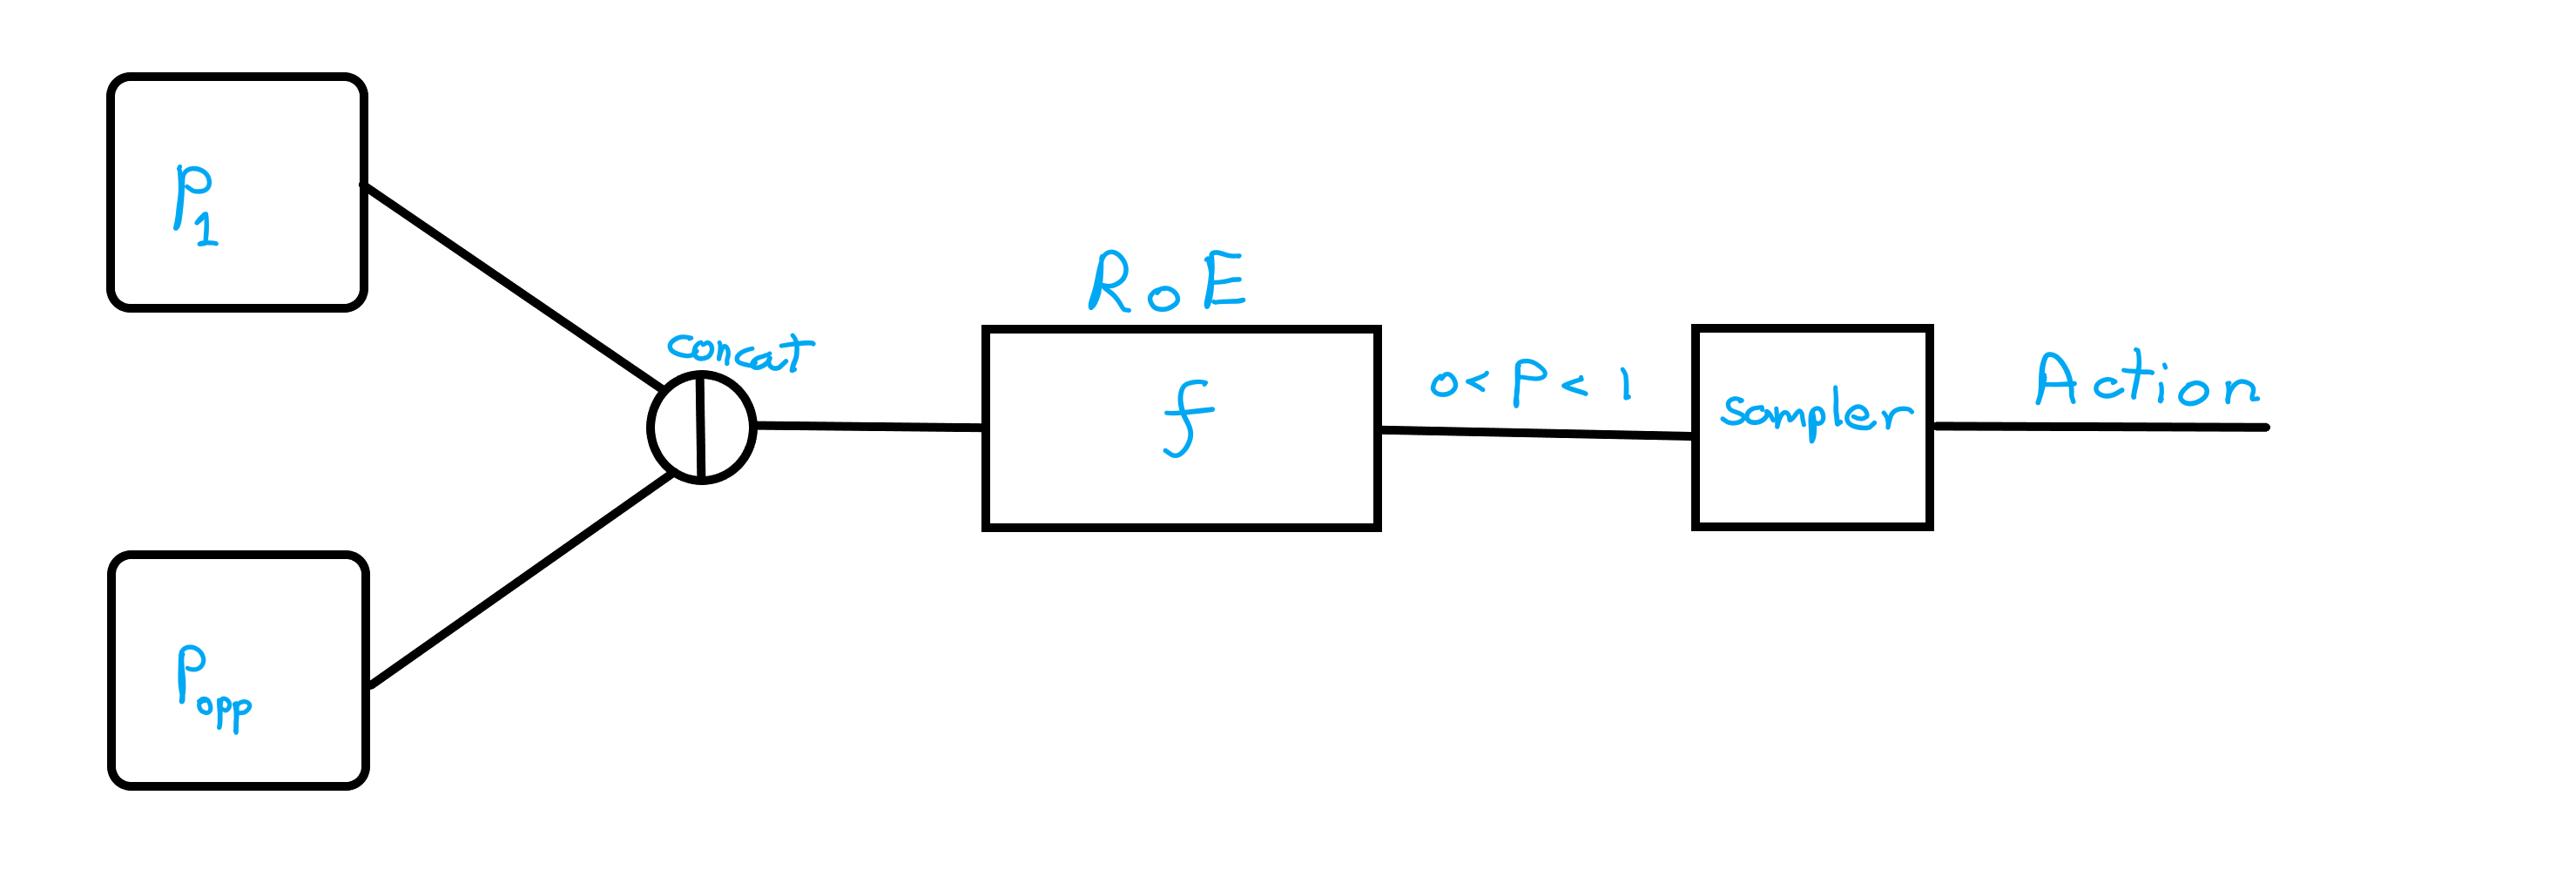
\includegraphics[scale=0.15]{Images/RoE.png}
                \caption{Depiction of a game with code of conduct}
            \end{figure}
        \end{frame}
        %----------------------------------------------------------
        \begin{frame}{Aritificial Neural Network}
            \begin{itemize}
                \item Parameterized function
                \item Can be tweaked by players
            \end{itemize}
            \begin{figure}[H]
                \centering
                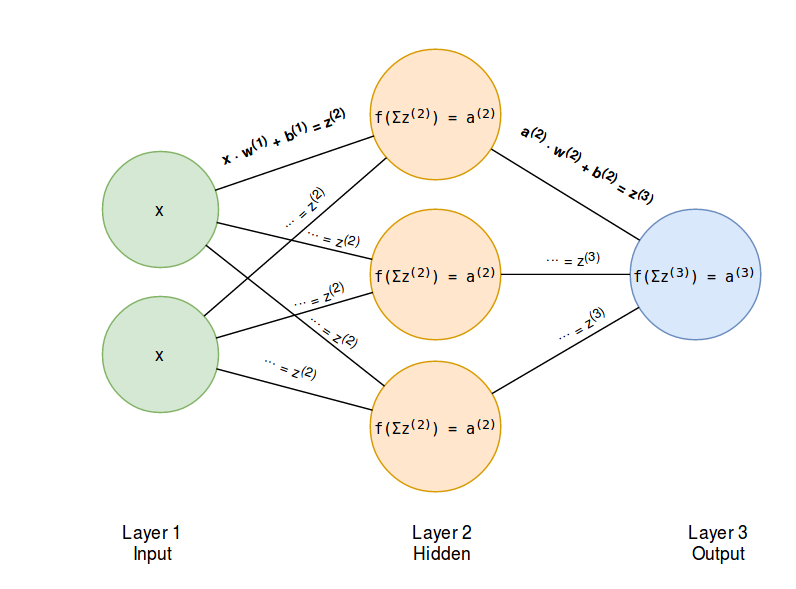
\includegraphics[scale=0.15]{Images/nn_diagram_1.png}
                \caption{Example neural network}
            \end{figure}
        \end{frame}

        %----------------------------------------------------------
        \begin{frame}{Playing one vs one}
        \begin{enumerate}
            \item Players are matched one on one randomly by Nature
            \item Players update RoE and display state through experience
        \end{enumerate}
            \begin{figure}[H]
                \centering
                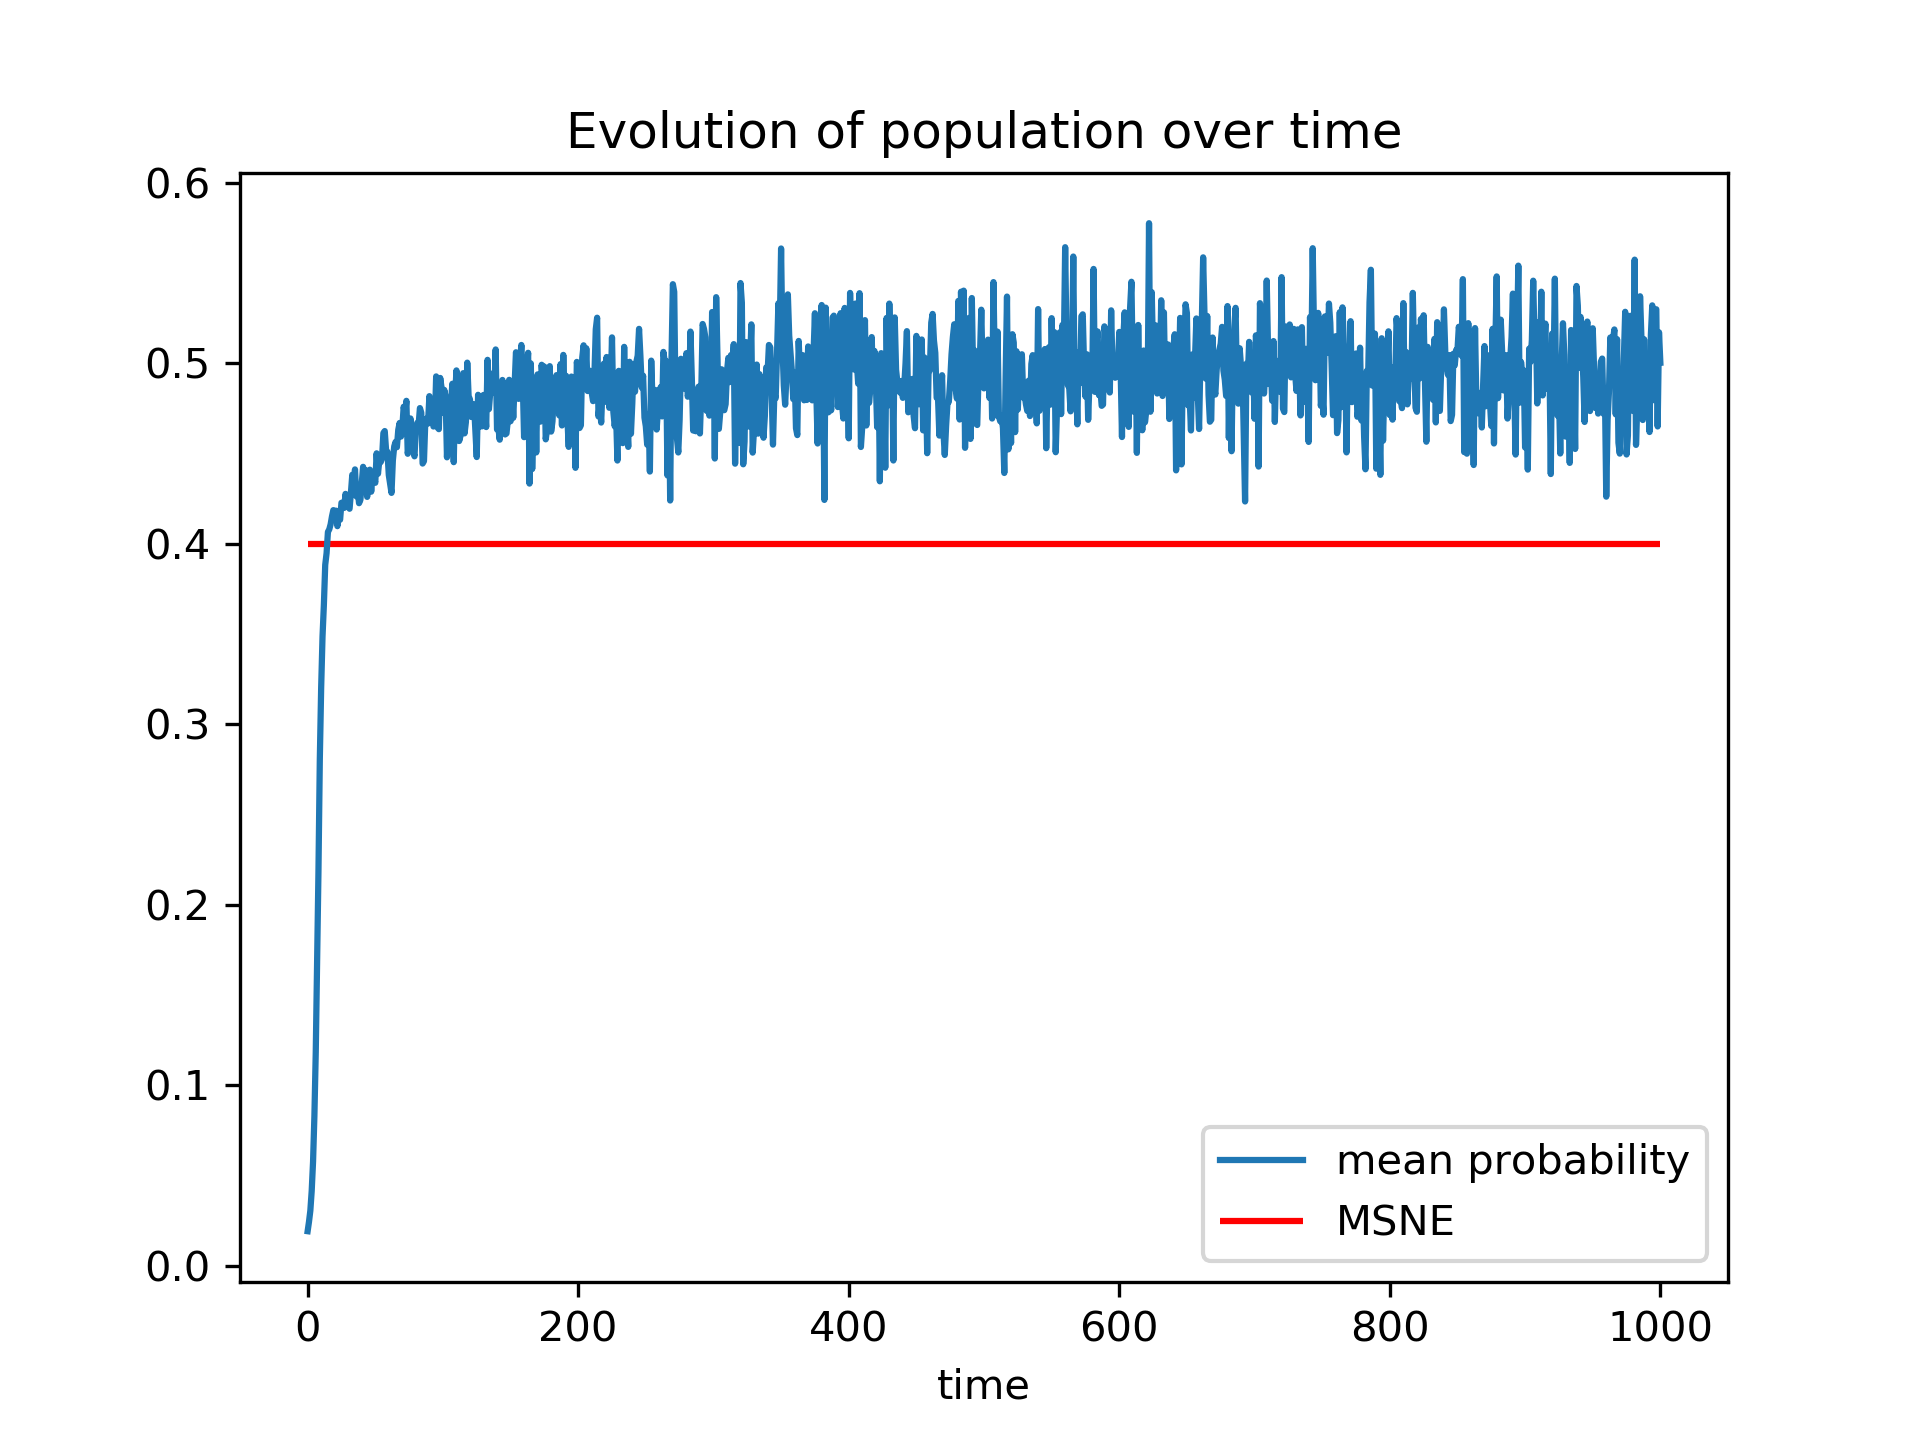
\includegraphics[scale=0.4]{Images/pop_state_uni.png}
                \caption{State of population (RoE) over time: pairwise contests. Some amount of inherent forced cooperation observed resulting in a population pay-off higher than MSNE}
            \end{figure}
        \end{frame}
                
        %----------------------------------------------------------
        \begin{frame}{Playing against the Field}
            \begin{itemize}
                \item Again, final population profile not MSNE.
                \item Lower variance during steady state.
            \end{itemize}
            \begin{figure}[H]
                \centering
                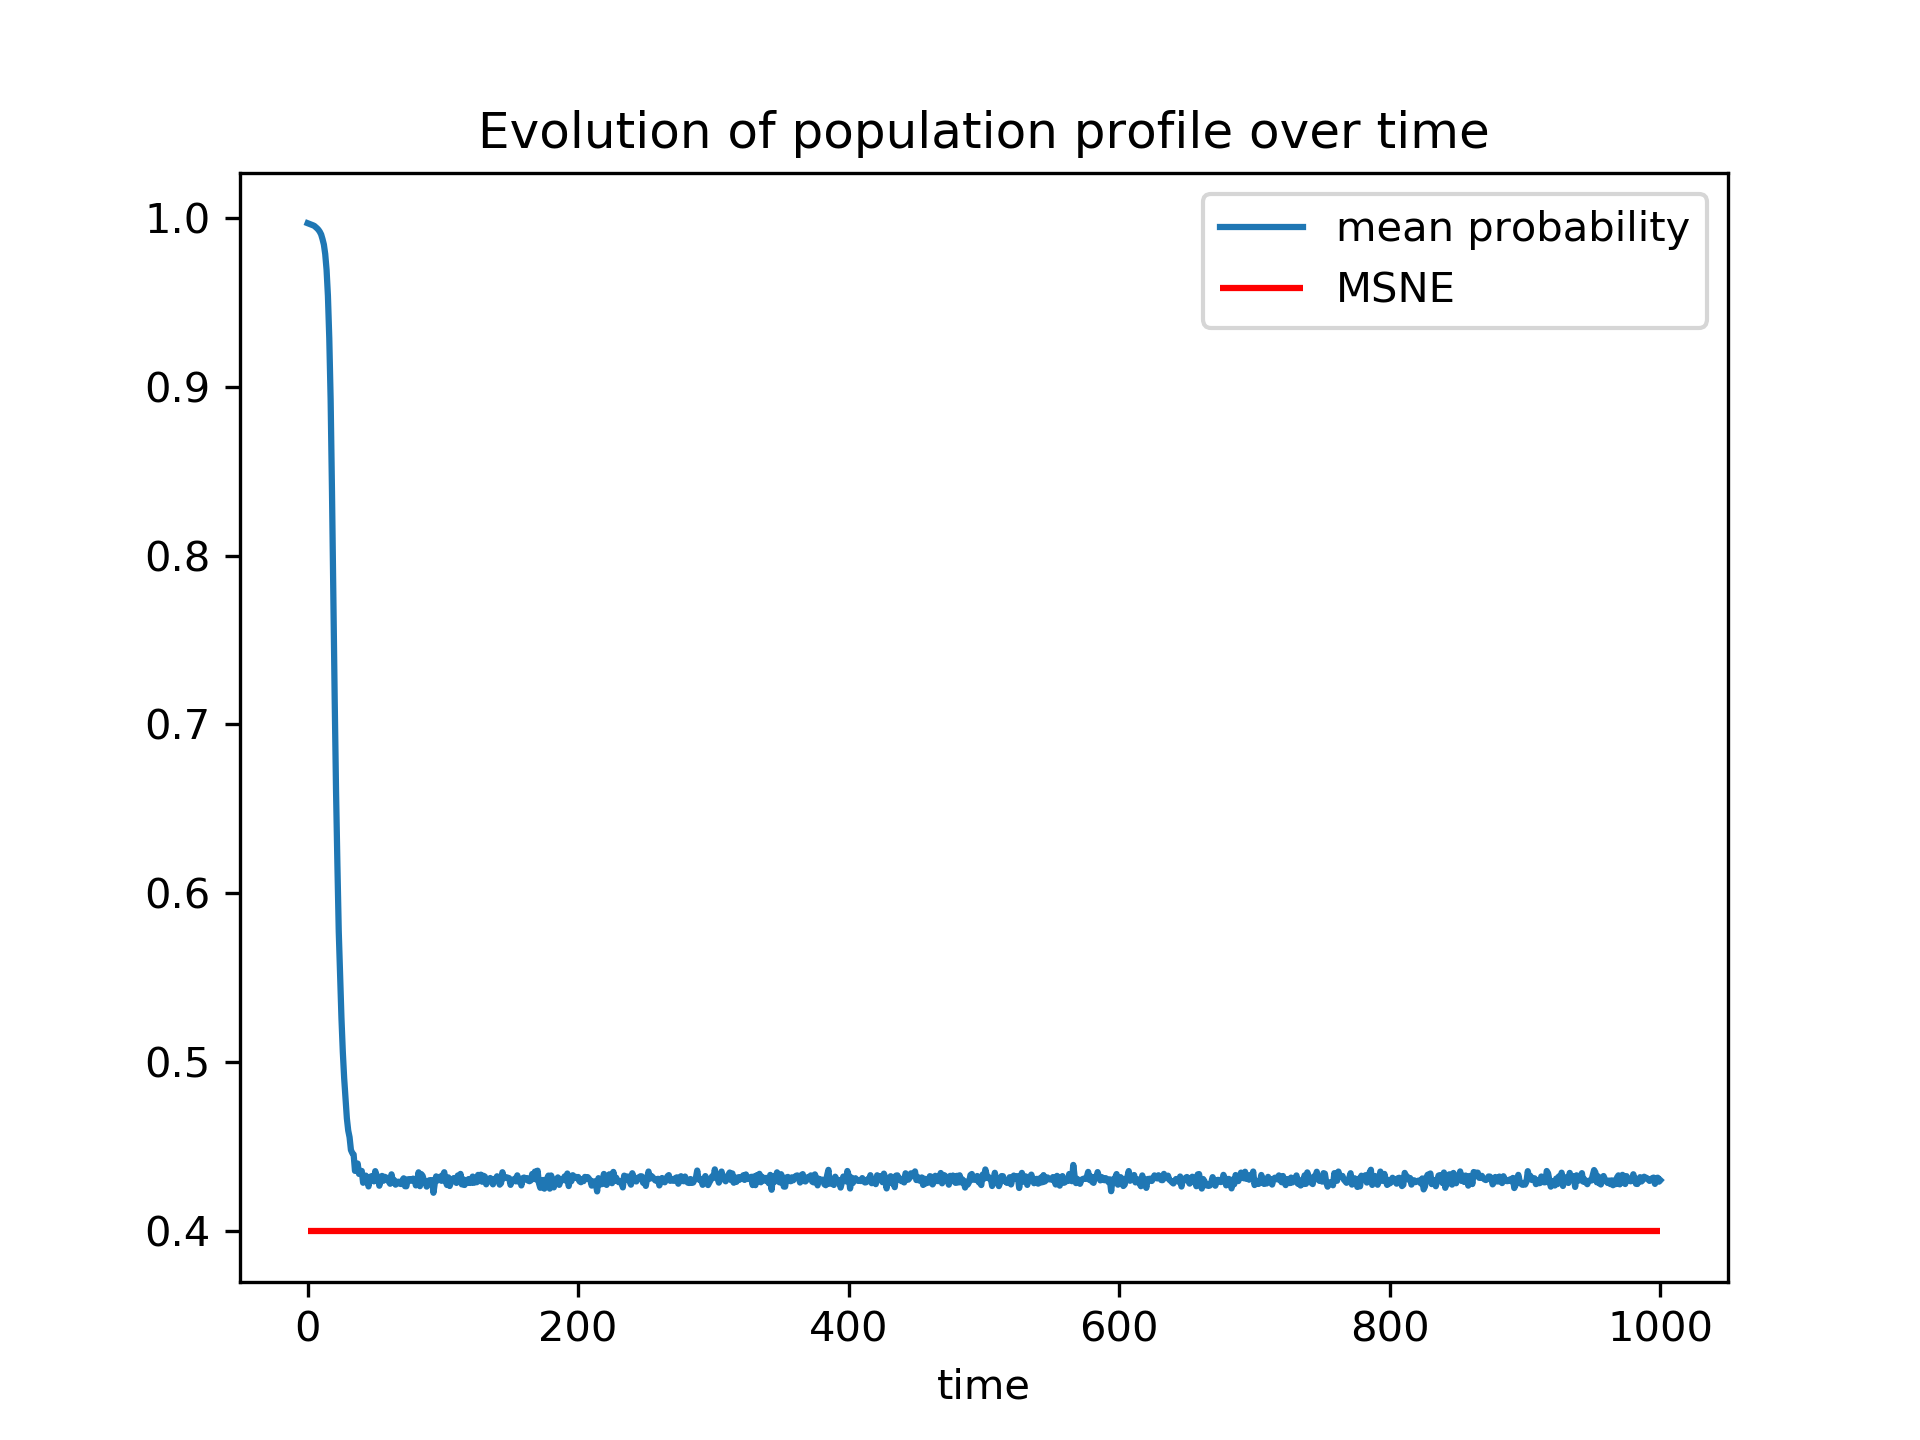
\includegraphics[scale=0.4]{Images/pop_state_uni_field.png}
                \caption{State of population (RoE) over time: against field. Some amount of inherent forced cooperation observed resulting in a population pay-off higher than MSNE}
            \end{figure}
        \end{frame}

    
        
    %$$$$$$$$$$$$$$$$$$$$$$$$$$$$$$$$$$$$$$$$$$$$$$$$$$$$$$$$$$$$$$
    \subsection{UCB Model}
        %----------------------------------------------------------
        \begin{frame}{Multi-Armed Bandits}
            \begin{itemize}
                \item A person must choose between multiple actions (originally comes from the idea of slot machines, the "one-armed bandits"), each with an unknown reward.
                \begin{figure}[H]
                    \centering
                    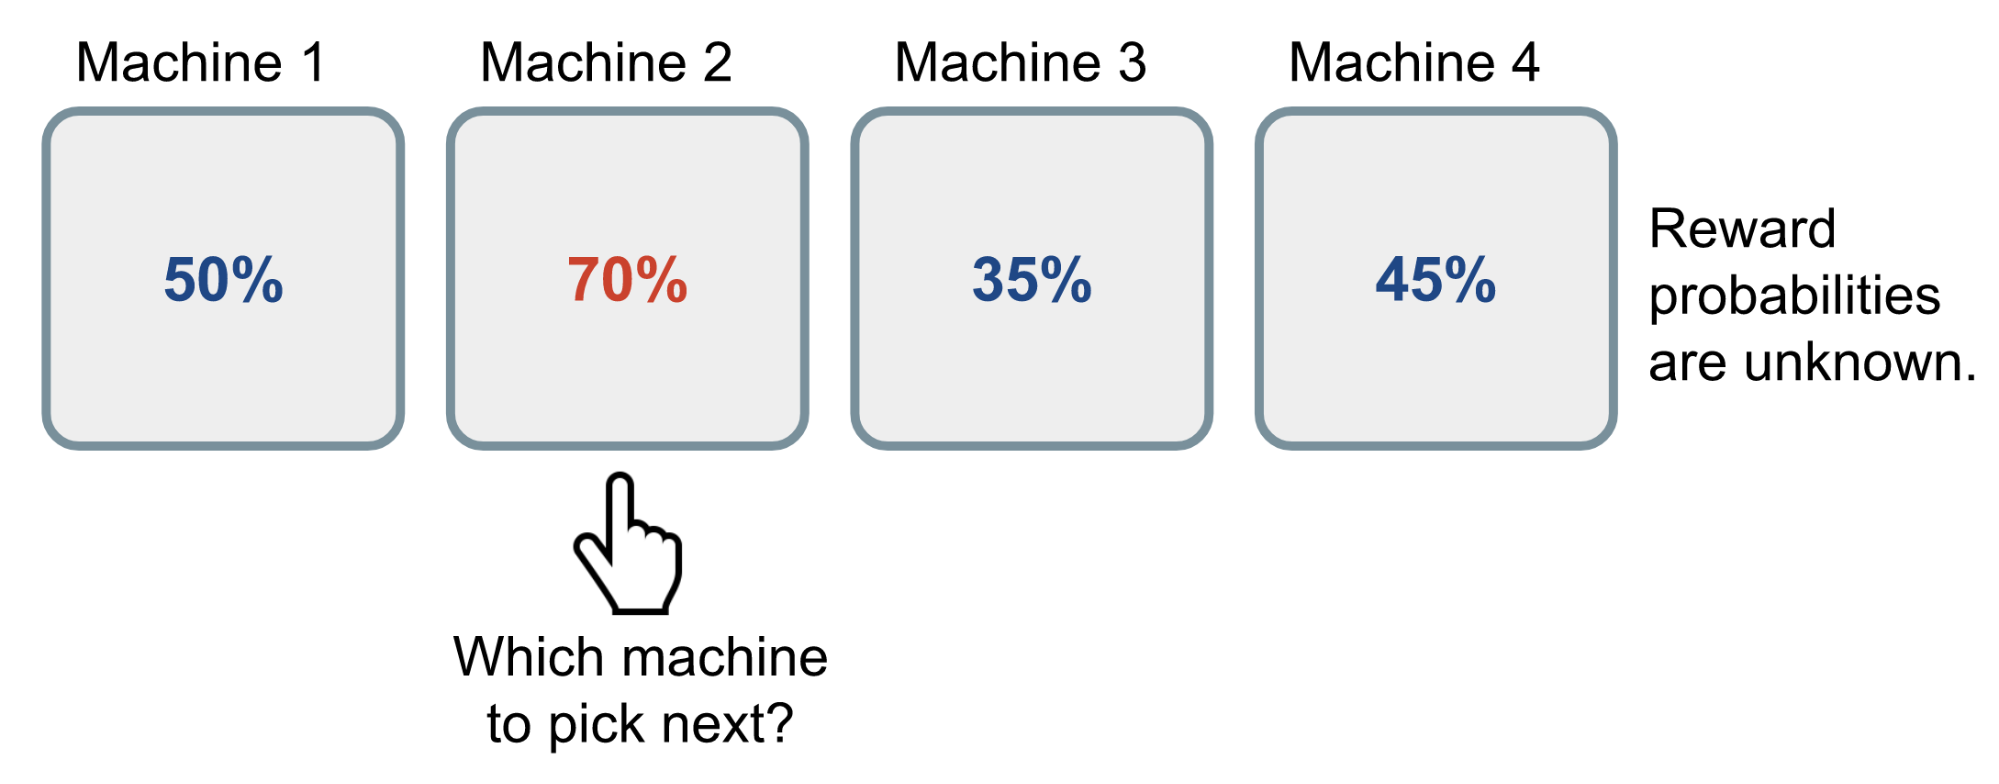
\includegraphics[scale=0.1]{Images/mab.png}
                    \caption{Multi-Armed Bandit Problem}
                    \label{fig:mab}
                \end{figure}
                \item Goal : determine the best or most profitable outcome through a series of choices.
                \item At the beginning of the experiment, when odds and payouts are unknown, the gambler must determine which machine to pull, in which order and how many times. 
            \end{itemize}
        \end{frame}

        %----------------------------------------------------------
        \begin{frame}{UCB Model}
        Upper Confidence Bound Algorithm :\\
        (For a single player)
            \begin{table}[H]
      			\centering
      			\begin{tabular}{ | c |}
        		\hline
        		\noindent Initialization: Play each arm once,\\\\
        		\noindent \textbf{For} t = K + 1, \dots , n, \textbf{repeat}\\\\
        		(1) Play arm $I_t = arg max_{k=1,...,K} UCB_t(k)$, where \\
        		$UCB_t(k) = \hat{\mu}_k(t-1) + \sqrt{\frac{8 \log t}{T_k (t-1)}}$\\\\
        		(2) Observe sample $X_t$ from the distribution $P_{I_{t}}$ \\
        		\noindent corresponding to the arm $I_t$.\\
        		\hline
			\end{tabular}
		\end{table}
        \end{frame}
        
        %----------------------------------------------------------
        \begin{frame}{Playing against Field}
            \begin{figure}
                \centering
                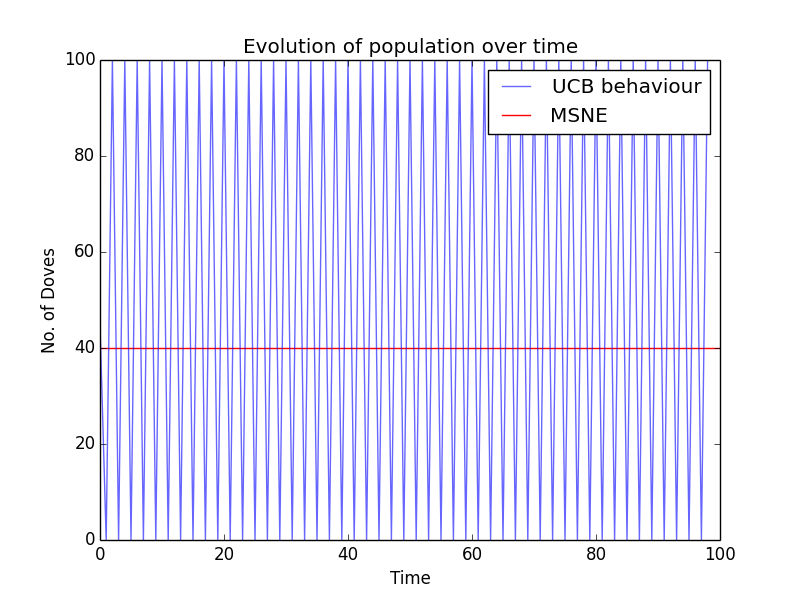
\includegraphics[scale=0.25]{Images/UCB/Population/full_100_100_epochs.png}
                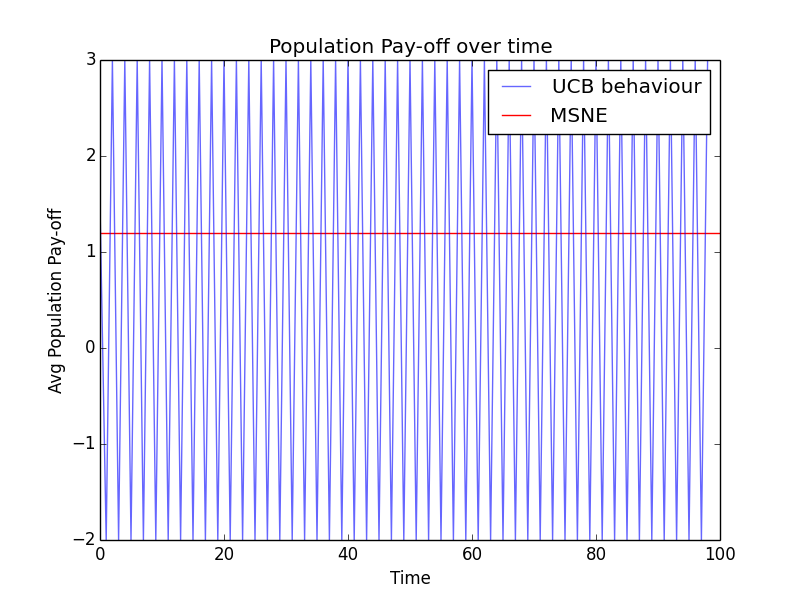
\includegraphics[scale=0.25]{Images/UCB/Pay-off/pay-off_full_100_100_epochs.png}
                \caption{Evolution of Population over time and the average pay-off of the population over time when the population is initialized randomly with probability 0.5 (Equivalent to individual pay-off over time after convergence in this case). \textbf{Each player interacts with everyone else in the population.}}
                \label{fig:my_label}
            \end{figure}
        \end{frame}
        
        %----------------------------------------------------------
        \begin{frame}{Playing against Field}
            \begin{figure}
                \centering
                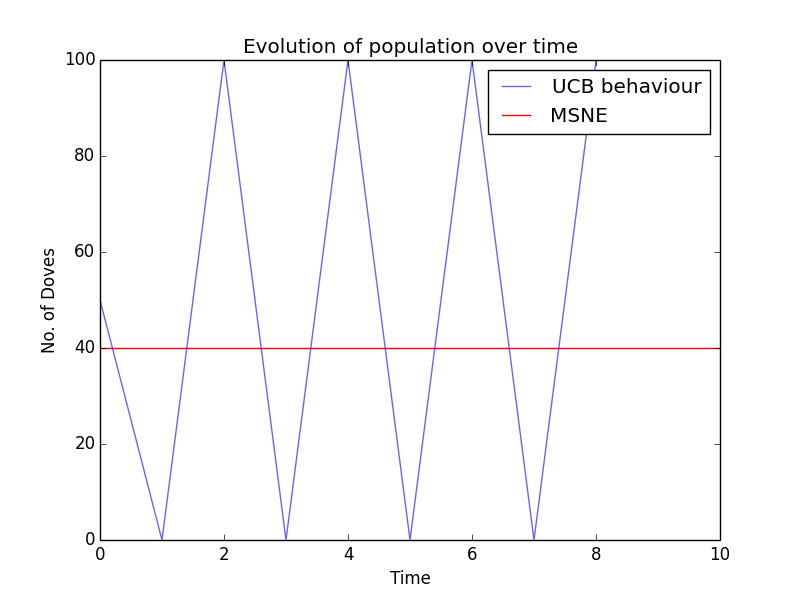
\includegraphics[scale=0.25]{Images/UCB/Population/full_100_10_epochs.png}
                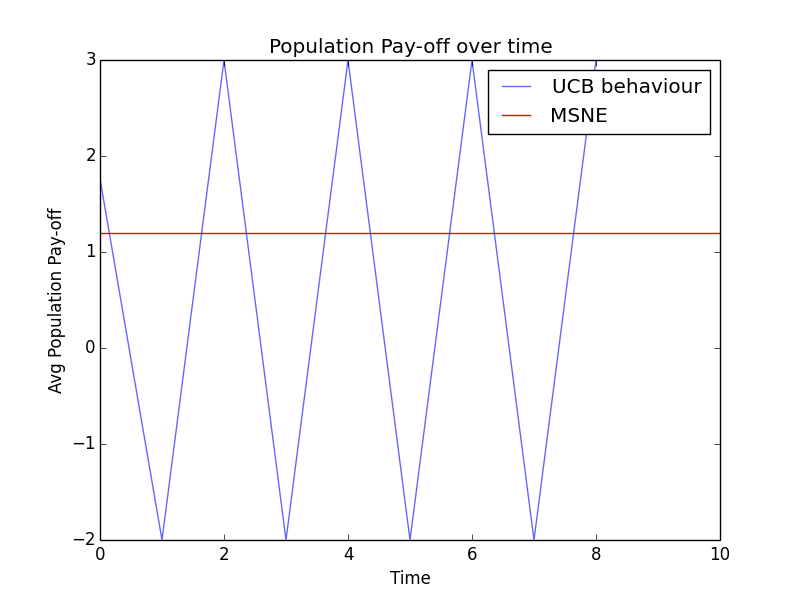
\includegraphics[scale=0.25]{Images/UCB/Pay-off/pay-off_full_100_10_epochs.png}
                \caption{Evolution of Population over time and the average pay-off of the population over time when the population is initialized randomly with probability 0.5 (Equivalent to individual pay-off over time after convergence in this case). \textbf{Each player interacts with everyone else in the population.}}
                \label{fig:my_label}
            \end{figure}
        \end{frame}
        
        %----------------------------------------------------------
        \begin{frame}{Playing Against a Group}
             \begin{figure}
                \centering
                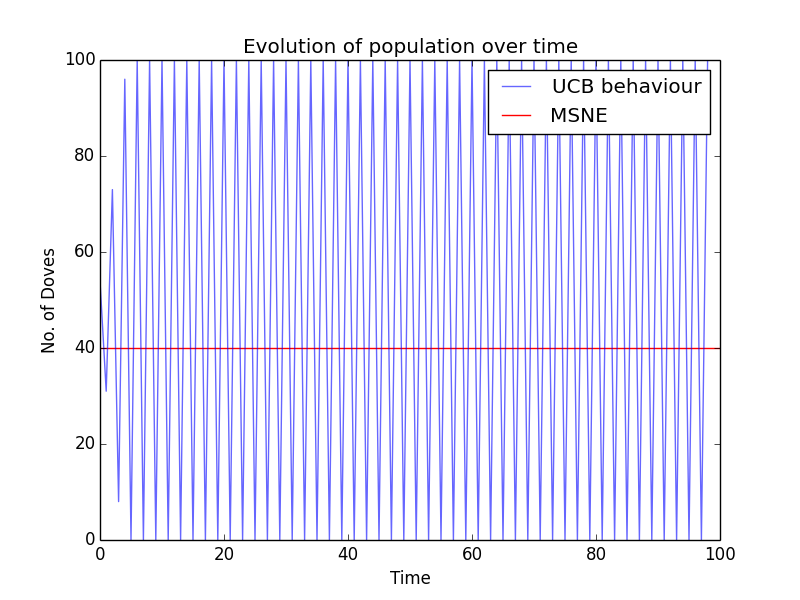
\includegraphics[scale=0.25]{Images/UCB/Population/mini_100_100_epochs.png}
                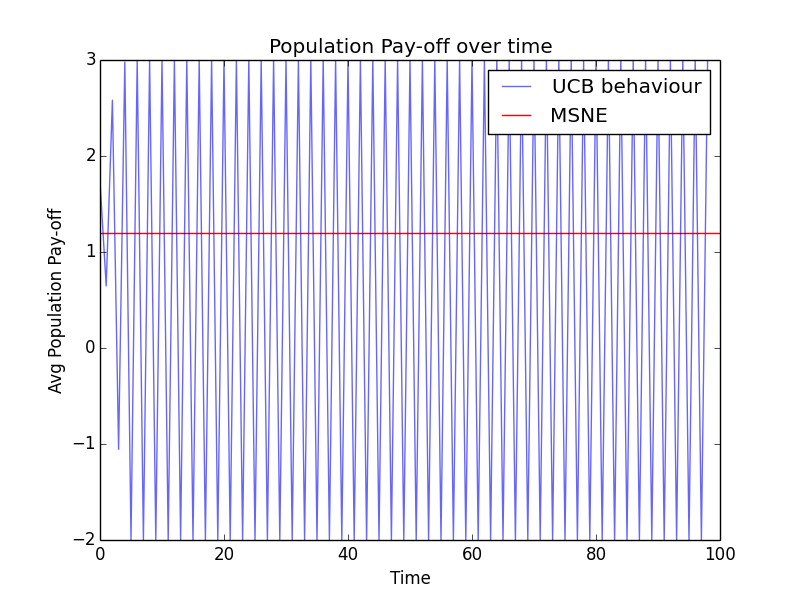
\includegraphics[scale=0.25]{Images/UCB/Pay-off/pay-off_mini_100_100_epochs.png}
                \caption{Evolution of Population over time and the average pay-off of the population over time when the population is initialized randomly with probability 0.5 (Equivalent to individual pay-off over time after convergence in this case). \textbf{Each player interacts with m<10$\%$ of the population.}}
                \label{fig:my_label}
            \end{figure}
        \end{frame}
        
        %----------------------------------------------------------
        \begin{frame}{Playing Against a Group}
             \begin{figure}
                \centering
                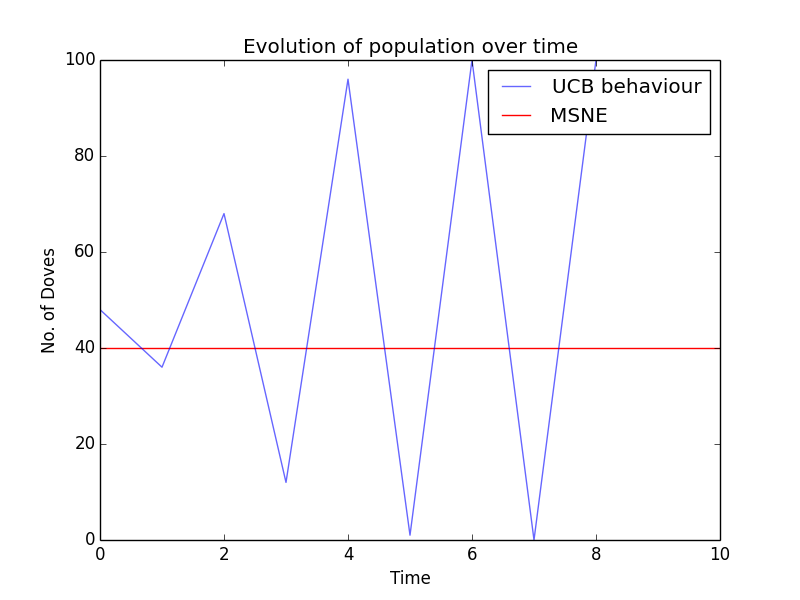
\includegraphics[scale=0.25]{Images/UCB/Population/mini_100_10_epochs.png}
                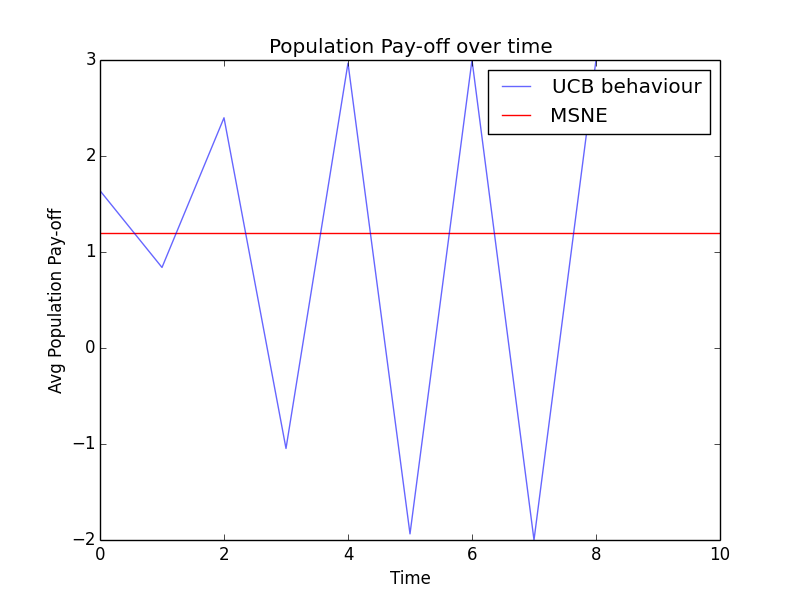
\includegraphics[scale=0.25]{Images/UCB/Pay-off/pay-off_mini_100_10_epochs.png}
                \caption{Evolution of Population over time and the average pay-off of the population over time when the population is initialized randomly with probability 0.5 (Equivalent to individual pay-off over time after convergence in this case). \textbf{Each player interacts with m<10$\%$ of the population.}}
                \label{fig:my_label}
            \end{figure}
        \end{frame}
        %----------------------------------------------------------
        \begin{frame}{Pair-wise contest}
            \begin{figure}
                \centering
                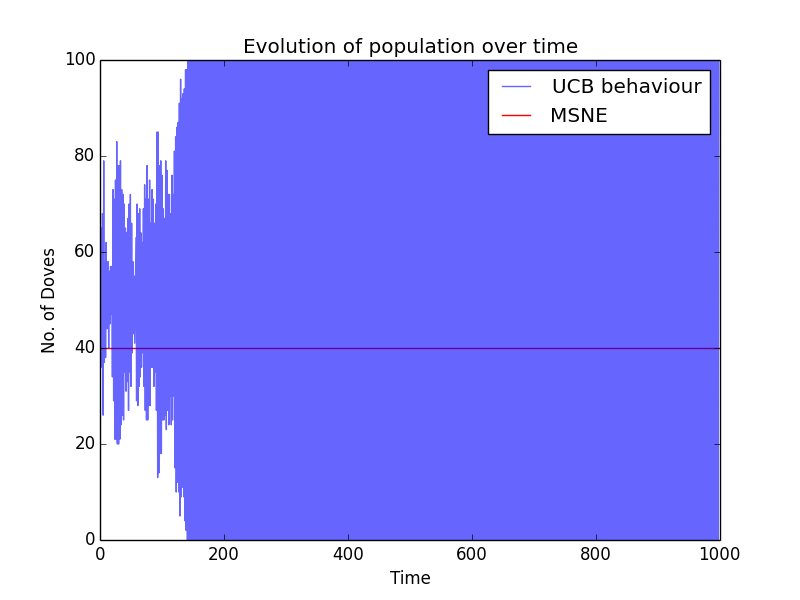
\includegraphics[scale=0.25]{Images/UCB/Population/pair_100_1000_epochs.png}
                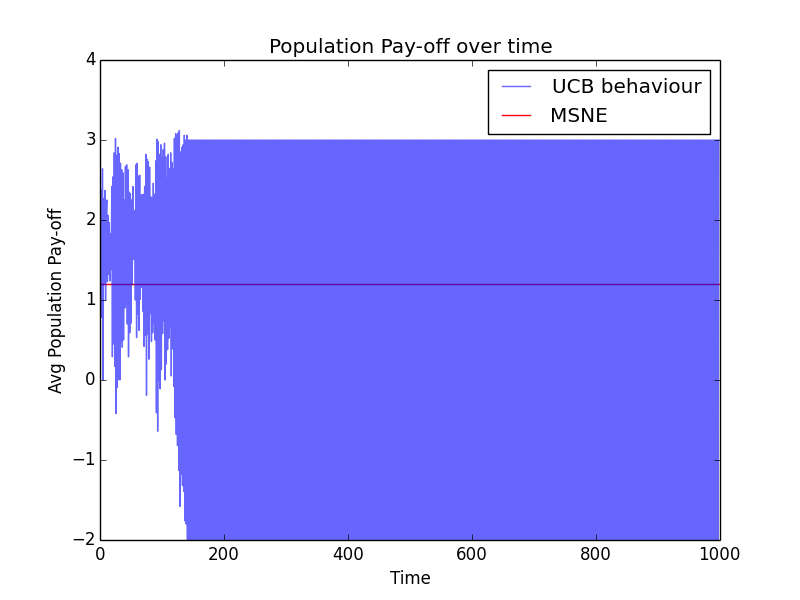
\includegraphics[scale=0.25]{Images/UCB/Pay-off/pay-off_pair_100_1000_epochs.png}
                \caption{Evolution of Population over time and the average pay-off of the population over time when the population is initialized randomly with probability 0.5 (Equivalent to individual pay-off over time after convergence in this case). \textbf{Every player interacts with another random player - one vs one.}}
                \label{fig:my_label}
            \end{figure}
        \end{frame}
        
        %----------------------------------------------------------
        \begin{frame}{Pair-wise contest}
            \begin{figure}
                \centering
                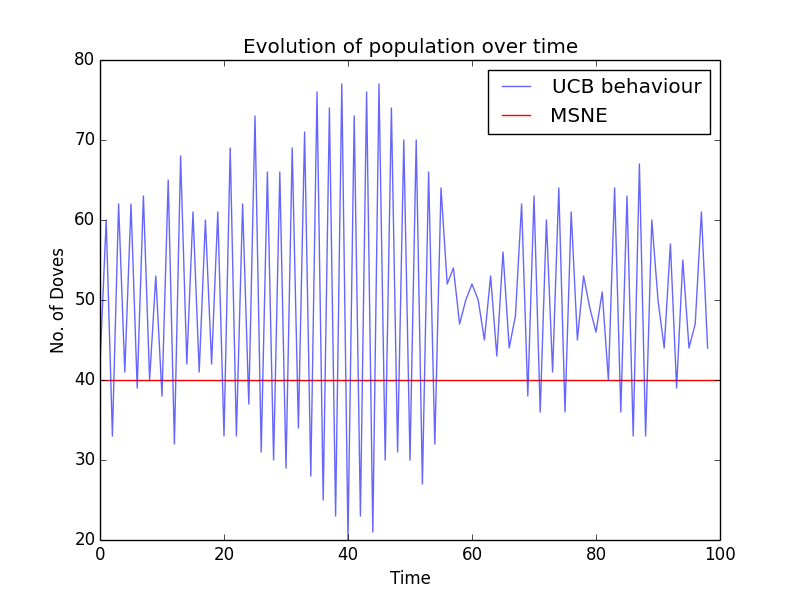
\includegraphics[scale=0.25]{Images/UCB/Population/pair_100_100_epochs.png}
                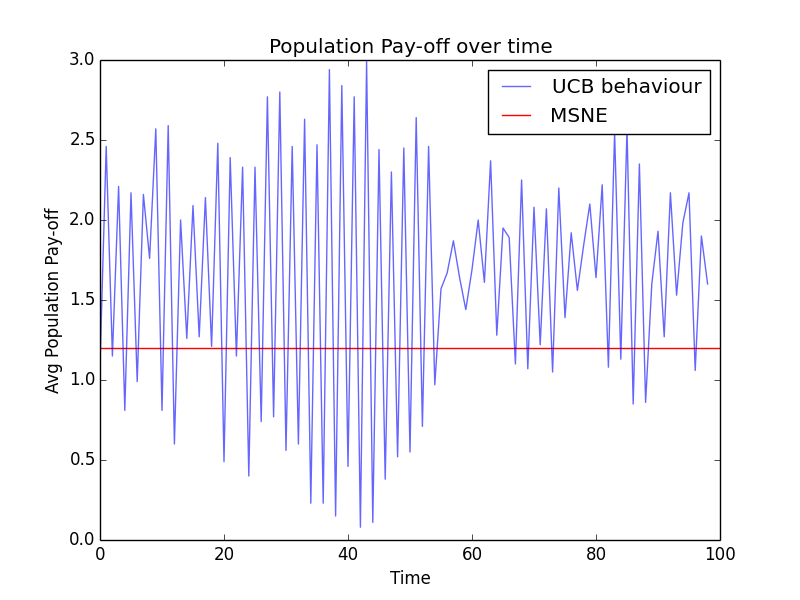
\includegraphics[scale=0.25]{Images/UCB/Pay-off/pay-off_pair_100_100_epochs.png}
                \caption{Evolution of Population over time and the average pay-off of the population over time when the population is initialized randomly with probability 0.5 (Equivalent to individual pay-off over time after convergence in this case). \textbf{Every player interacts with another random player - one vs one.}}
                \label{fig:my_label}
            \end{figure}
        \end{frame}
        
        %----------------------------------------------------------
        \begin{frame}{A better understanding of its significance during convergence}
            \begin{figure}[H]
                \centering
                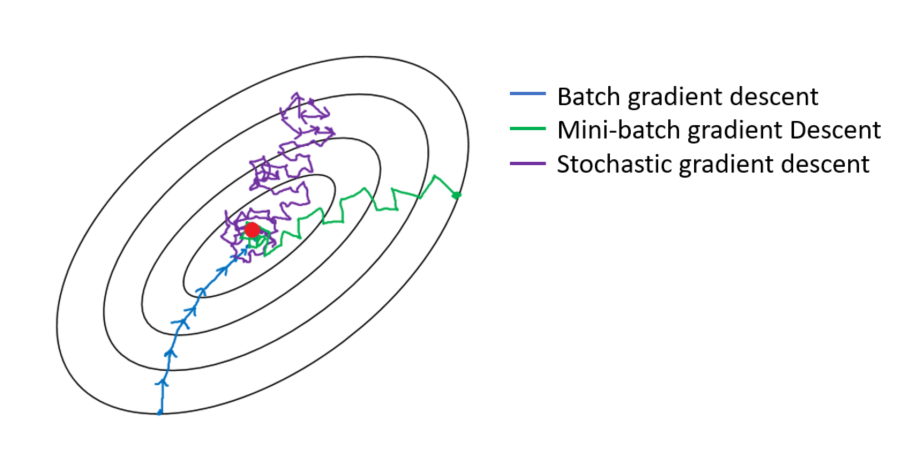
\includegraphics[scale=0.25]{Images/GD.png}
                \caption{Convergence comparison of the three methods of calculating individual pay-offs : Playing against the field, Playing against a group and Pair-wise contest respectively}
                \label{fig:GD}
            \end{figure}
        \end{frame}
        
        
        %----------------------------------------------------------
        \begin{frame}{Summarizing UCB experiments}
            \begin{itemize}
                \item Observations :
                    \begin{itemize}
                        \item In all 3 cases, the population converges to a cycle (either all Hawk or all Dove)
                        \item In all 3 cases, the average population pay-off converges to a cycle (either -2 or +3)
                        \item The convergence rate of the 3 methods similar to Full Batch GD, Mini Batch GD and SGD\\\\
                    \end{itemize}
                \item Inference :
                    \begin{itemize}
                        \item Playing against Field : When majority of the \emph{current} population is Dove(>40$\%$), better to be a Hawk.
                        \item Playing Against a Group : When majority of the \emph{sampled} population is Dove(>40$\%$), better to be a Hawk
                        \item Pair-wise contest : When \emph{he}'s a Dove, I'm better off as Hawk
                    \end{itemize}
                \item Reason :
                    \begin{itemize}
                        \item \textbf{Each player in each iteration chooses best response}
                    \end{itemize}
            \end{itemize}
        \end{frame}
        
                %----------------------------------------------------------
        \begin{frame}{Group Play}
            \begin{figure}
                \centering
                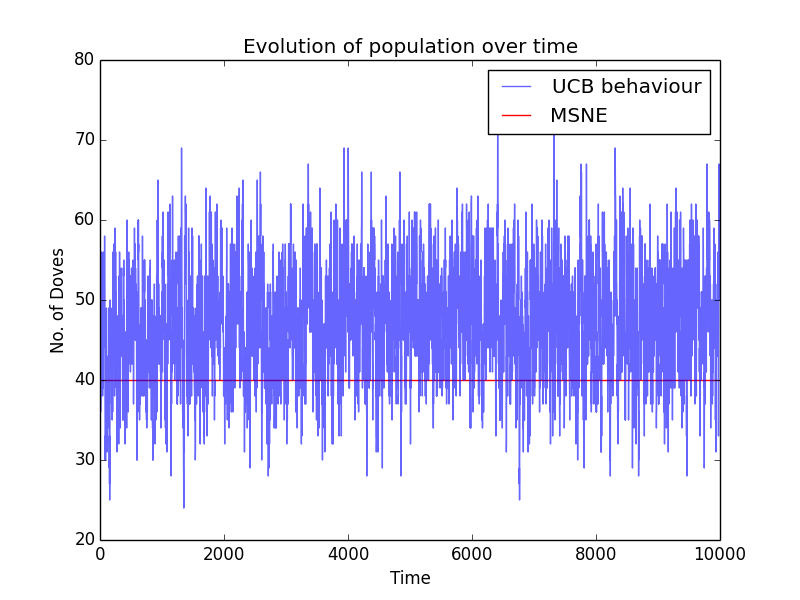
\includegraphics[scale=0.25]{Images/UCB/Population/group_100_10000_epochs.png}
                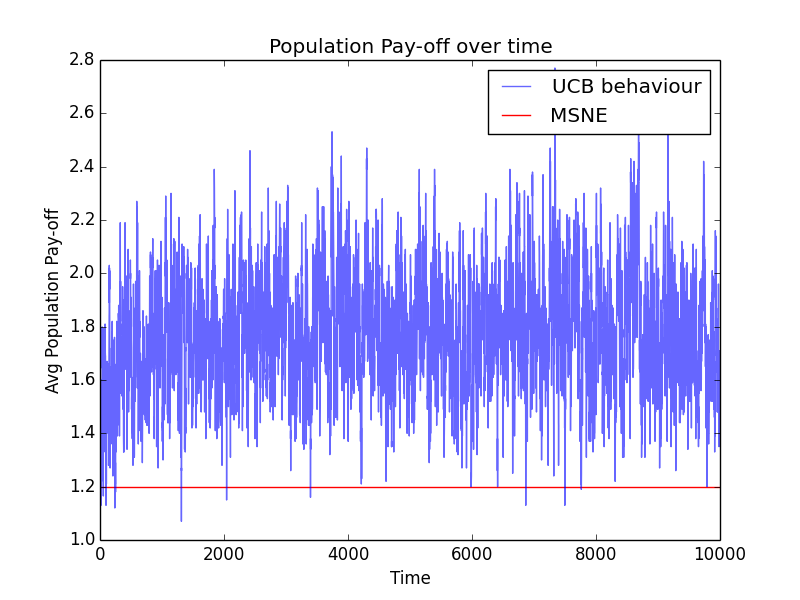
\includegraphics[scale=0.25]{Images/UCB/Pay-off/pay-off_group_100_10000_epochs.png}
                \caption{Evolution of Population over time and the average pay-off of the population over time when the population is initialized randomly with probability 0.5. \textbf{A group of m=10$\%$ of the population interacts in each interaction.}}
                \label{fig:my_label}
            \end{figure}
        \end{frame}
        
                %----------------------------------------------------------
        \begin{frame}{Group Play}
            \begin{figure}
                \centering
                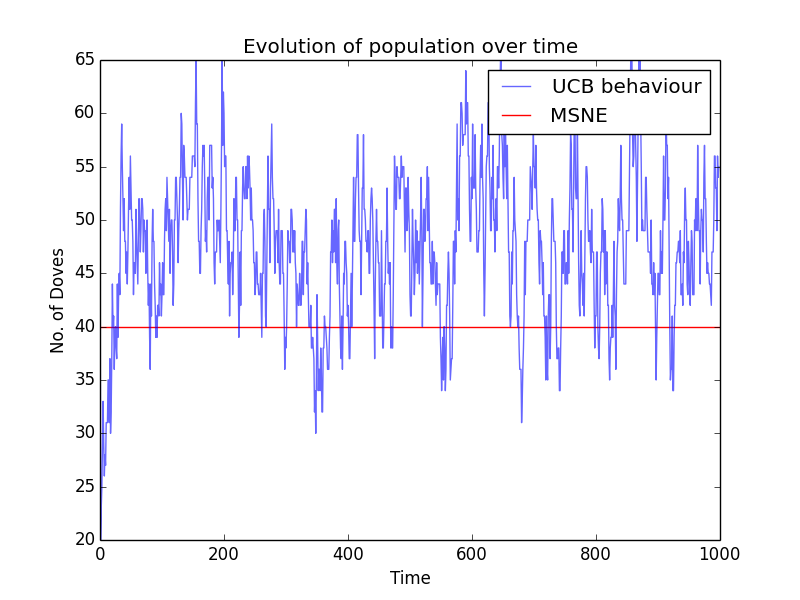
\includegraphics[scale=0.25]{Images/UCB/Population/group_100_1000_epochs.png}
                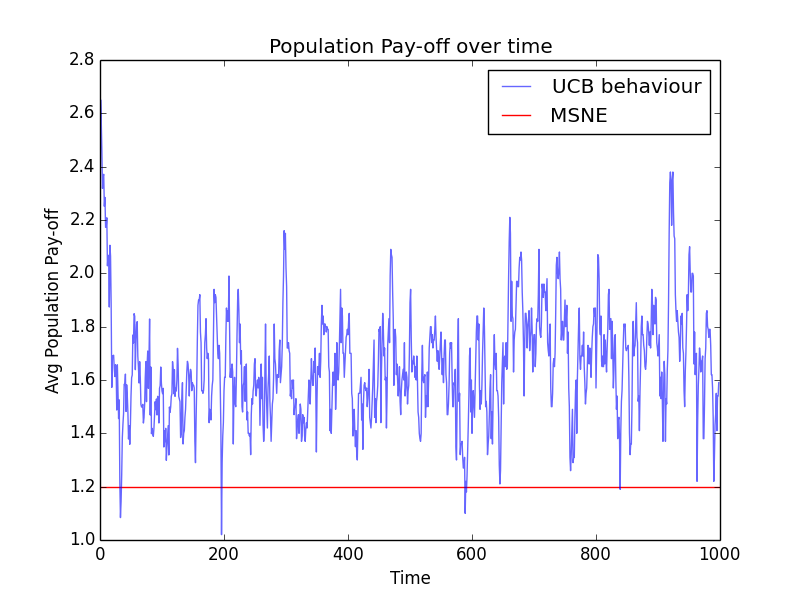
\includegraphics[scale=0.25]{Images/UCB/Pay-off/pay-off_group_100_1000_epochs.png}
                \caption{Evolution of Population over time and the average pay-off of the population over time when the population is initialized randomly with probability 0.5. \textbf{A group of m=10$\%$ of the population interacts in each interaction.}}
                \label{fig:my_label}
            \end{figure}
        \end{frame}
        
        %----------------------------------------------------------
        \begin{frame}{Group Play}
            \begin{itemize}
                \item Observation :
                    \begin{itemize}
                        \item Fairly robust to different population initialization techniques :\\
                            \begin{table}[H]
                              \begin{center}
                                \begin{tabular}{|c|c|c|} % <-- Alignments: 1st column left, 2nd middle and 3rd right, with vertical lines in between
                                \hline
                                Initialization & Avg No. of Dove & Avg population pay-off\\
                                  \hline
                                  All Hawk & 48 & 1.76 \\
                                  \hline
                                  All Dove & 47 & 1.78 \\
                                  \hline
                                  Random (p=0.5) & 47 & 1.78 \\
                                  \hline
                                \end{tabular}
                              \end{center}
                            \end{table}
                        \item Average population pay-off better than MSNE pay-off
                    \end{itemize}
                \item Reason :
                    \begin{itemize}
                        \item The change in population distribution is minimal
                    \end{itemize}
            \end{itemize}
        \end{frame}

%%%%%%%%%%%%%%%%%%%%%%%%%%%%%%%%%%%%%%%%%%%%%%%%%%%%%%%%%%%%%%%%%%%%%%
\section{Future Work}
    %----------------------------------------------------------
    \begin{frame}{Future Work}
        \begin{itemize}
            \item Asymmetric Games (eg) Trust-Cooperate
            \item Strange attractors to analyse chaotic populations
            % \item Evolutionary Programming
            \item Quantifying rewards of cooperation
            \item  Informed Reinforcement learners : use communication through revelation schemes
        \end{itemize}
    \end{frame}

%%%%%%%%%%%%%%%%%%%%%%%%%%%%%%%%%%%%%%%%%%%%%%%%%%%%%%%%%%%%%%%%%%%%%%
\section{Previous Works}
    %----------------------------------------------------------
    \begin{frame}{Axelrod - Evolution of Cooperation}
        \begin{itemize}
            \item Also used to analyze behavior of populations
            \item made use of evolutionary programming
        \end{itemize}
        \begin{figure}
            \centering
            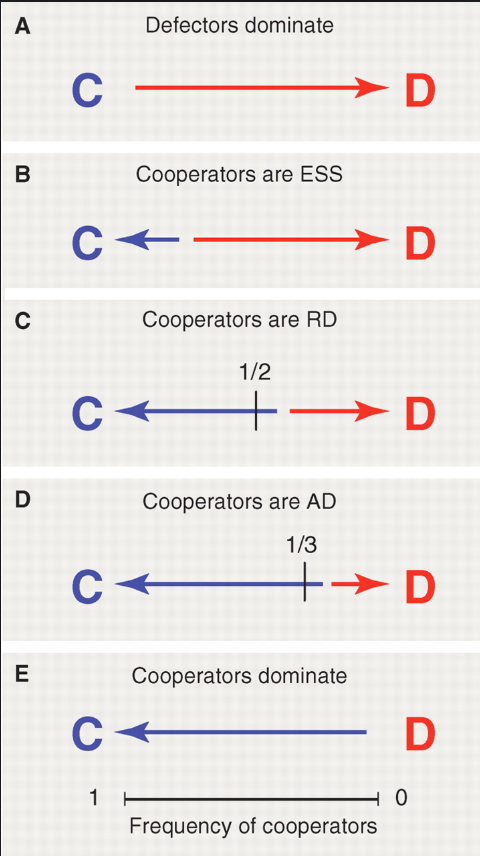
\includegraphics[scale=0.25]{Images/evolution_coop.png}
            \caption{5 stages of the evolution of cooperation}
        \end{figure}
    \end{frame}


    %----------------------------------------------------------
    \begin{frame}{Evolutionary Game Theory and Multi-Agent Reinforcement Learning}
    \begin{itemize}
        \item Authors :  Karl Tuyls and Ann Nowe
        \item Survey the basics of RL and (Evolutionary) Game Theory
        \item Multi-Agent Systems
        \item Mathematical connection between MARL and Evolutionary Game Theory
        \item Ref : \href{https://pdfs.semanticscholar.org/bb9f/bee22eae2b47bbf304804a6ac07def1aecdb.pdf}{\emph{Paper pdf}}
    \end{itemize}
    \end{frame}

    % %----------------------------------------------------------
    %     \begin{frame}{Evolutionary Stable Strategies}
    %         \begin{itemize}
    %             \item Solution concept for N-player games
    %             \item No guaranteed existence (eg) Rock-Paper-Scissors
    %             \item Always a Nash equilibrium
    %         \end{itemize}
    %         \begin{figure}[H]
    %             \centering
    %             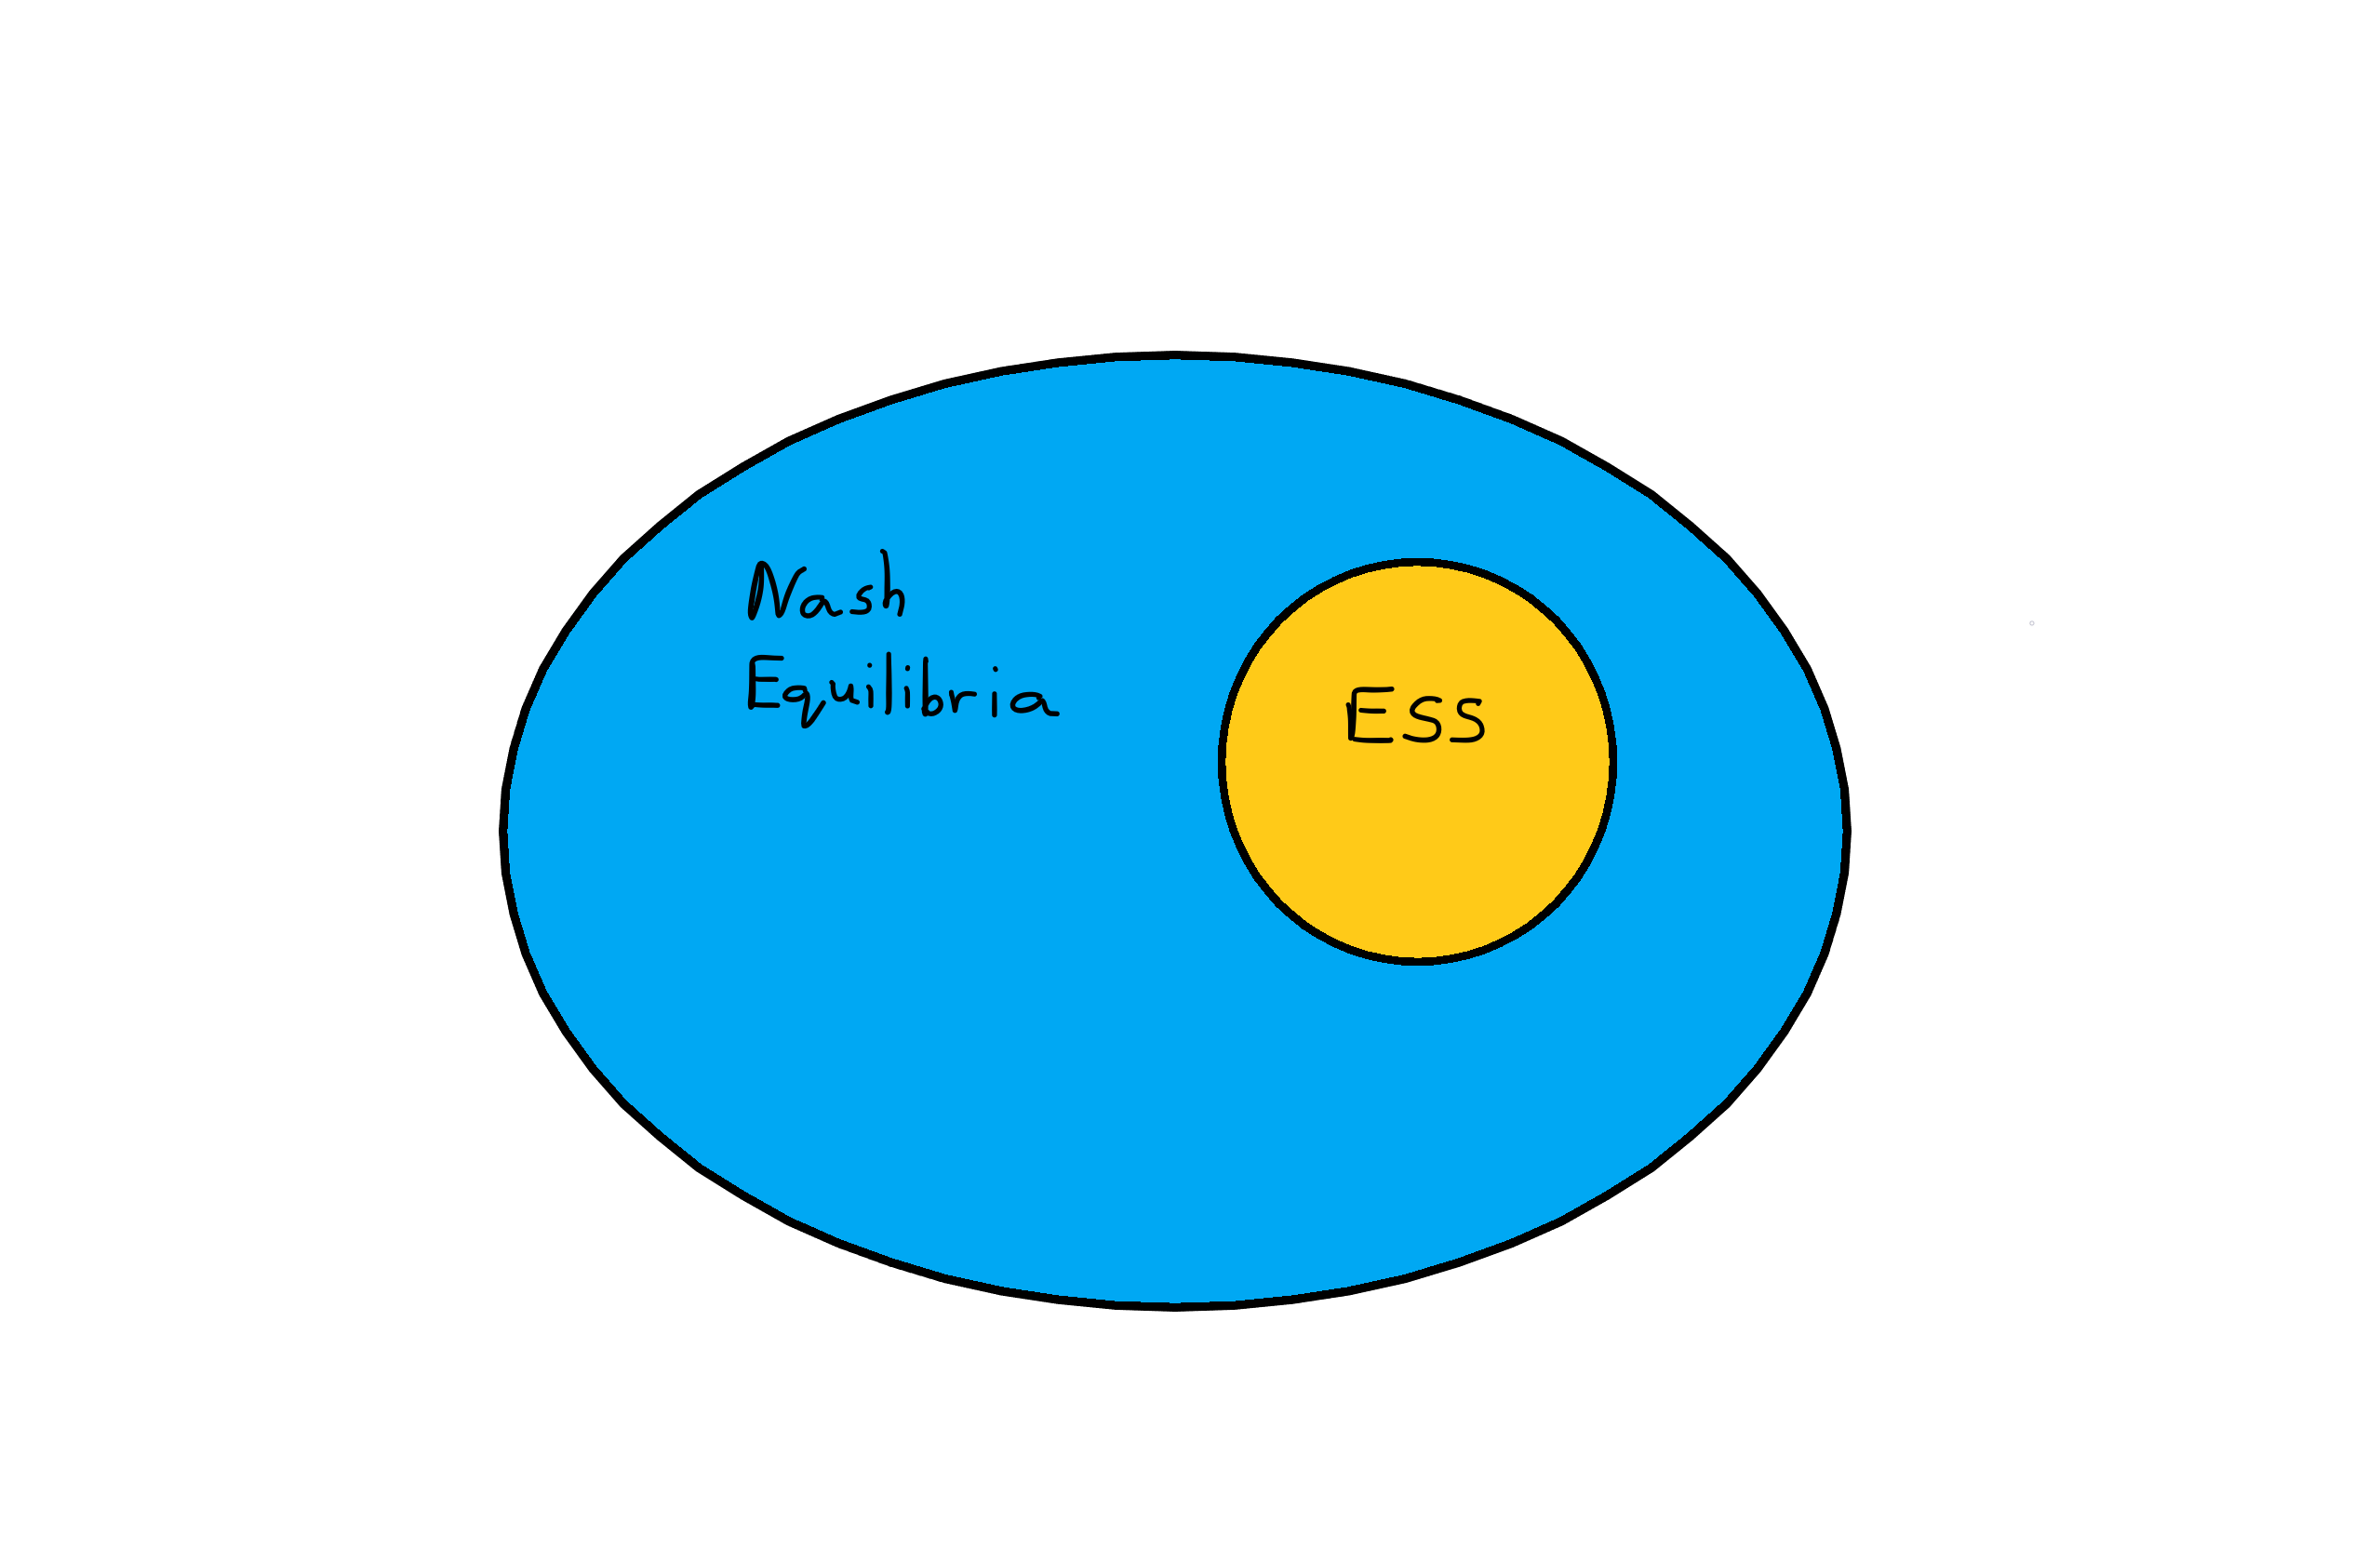
\includegraphics[scale=0.1]{Images/nashess.png}
    %             \caption{Relation between Nash Equilibria and ESS}
    %         \end{figure}
    %     \end{frame}
    
%%%%%%%%%%%%%%%%%%%%%%%%%%%%%%%%%%%%%%%%%%%%%%%%%%%%%%%%%%%%%%%%%%%%%%
\section{References}
    %----------------------------------------------------------
    \nocite{DBLP:books/lib/SuttonB98, Barker2017}
    \begin{frame}{References}
        \printbibliography
    \end{frame}

    \begin{frame}{ }
        \begin{center}
            \Huge{\weva{\textbf{THANK YOU }}
            \textbf{:)}}
        \end{center}
        
    \end{frame}

\end{document}
